% -*- coding: utf-8; -*-

\chapter{Revisão Bibliográfica}

Neste capitulo, são apresentadas primeiramente a importância
econômica, formação, composição e estrutura interna do material a ser
estudado.  A seguir são revisadas as técnicas de MD, relevantes no
contexto deste trabalho, no âmbito da microscopia ótica de luz
refletida e da análise de imagens.

\section{Minério de Ferro}

O ferro é um dos elementos mais abundantes da crosta terrestre (o
segundo metal, com aproximadamente 4,2\%) e matéria-prima fundamental
para a indústria.

O maior desenvolvimento de formação ferrífera ocorreu no período
Pré-cambriano tardio da era Proterozóica. Estas formações ocorreram
nas rochas sedimentares do tipo Formações Ferríferas Bandadas (BIF -
\textit{Banded Iron Formation}).\cite{15,16} As BIF estão compostas
por grandes depósitos de camadas ricas em ferro, alternando com
camadas ricas em silício. Elas representam os maiores depósitos de
minério de ferro do planeta.\cite{17}

Os maiores depósitos de minério de ferro, no Brasil, são praticamente
todos do tipo hematítico, com altos teores de ferro.\cite{18} As
reservas medidas e indicadas de minério de ferro no Brasil alcançam 29
bilhões de toneladas (Tabela~\ref{tab:2-1}), situando o país em
segundo lugar em relação às reservas mundiais, de 166 bilhões de
toneladas.\cite{19}

% -*- coding: utf-8; -*-

\begin{table} [!h]
 \begin{center}  \footnotesize
  \caption{Reservas mundiais de minério de ferro no ano 2011 ($10^{6}$~t).\cite{19}} \label{tab:2-1}
  ~\\[-1mm]
   \begin{tabularx}
     {0.83\textwidth}
     { p{3.5cm}
       @{}n{5}{1}
       @{\extracolsep{8mm}}n{4}{1}
       @{\extracolsep{12mm}}n{5}{1}
       @{\extracolsep{8mm}}n{4}{1} }

   \textbf{Países}
   & \textbf{RM}$^\dag$
   & \textbf{RM [\%]}
   & \textbf{RC}
   & \textbf{RC [\%]} \\ \toprule

   ~\\[-2mm]
   Austrália
   & 35000
   & 21.08
   & 17000
   & 21.25 \\ \midrule

   Brasil
   & 29000
   & 17.47
   & 16000
   & 20.00 \\ \midrule


   Rússia
   & 25000
   & 15.06
   & 14000
   & 17.50 \\ \midrule

   China
   & 23000
   & 13.86
   & 7200
   & 9.00 \\ \midrule

   Índia
   & 7000
   & 4.22
   & 4500
   & 5.62 \\ \midrule

   Estados Unidos
   & 6900
   & 4.16
   & 2100
   & 2.62 \\ \midrule

   Canadá 
   & 6300
   & 3.80
   & 2300
   & 2.88 \\ \midrule

   Ucrânia
   & 6000
   & 3.61
   & 2100
   & 2.62 \\ \midrule

   Venezuela 
   & 4000
   & 2.41
   & 2400
   & 3.00 \\ \midrule
   
   Suécia  
   & 3500
   & 2.11
   & 2200
   & 2.75 \\ \midrule
   
   Cazaquistão 
   & 3000
   & 1.81
   & 1000
   & 1.25 \\ \midrule
   
   Irã 
   & 2500
   & 1.51
   & 1400
   & 1.75 \\ \midrule   
   
   Mauritânia
   & 1100
   & 0.66
   & 700
   & 0.88 \\ \midrule 
   
   África do Sul 
   & 1000
   & 0.60
   & 650
   & 0.81 \\ \midrule    
   
   México
   & 700
   & 0.42
   & 400
   & 0.50 \\ \midrule   
   
   Outros países
   & 12000
   & 7.23
   & 6000
   & 7.50 \\ \midrule 
   
   \textbf{TOTAL}
   & 166000
   & 100.00
   & 80000
   & 100.00 \\          

  \end{tabularx}
 \end{center}
 {$^\dag$ \scriptsize RM: Reservas Medidas; RC: Reservas Contidas}
\end{table}

Entretanto, em termos de ferro contido, as reservas brasileiras têm
teor médio muito alto (aproximadamente 55\%) e, embora continue em
segundo, fica muito mais próximo do primeiro lugar internacional. Esse
fato ocorre devido ao alto teor de ferro encontrado nas hematitas
(60\% a 67\% de ferro), predominante no Pará, e itabirito (50\% a 60\%
de ferro), predominante em Minas Gerais.\cite{20}

% -*- coding: utf-8; -*-

\begin{table} [!h]
 \begin{center}  \footnotesize
  \caption{Reservas brasileiras de minério de ferro Medidas e Indicadas (em toneladas).\cite{21}} \label{tab:2-2}
  ~\\[-1mm]
   \begin{tabularx}
     {0.95\textwidth}
     { p{1.3cm}
       p{4.6cm}
       @{}n{11}{1}
       @{\extracolsep{2mm}}n{6}{1}
       @{\extracolsep{6mm}}n{4}{1} }

   \textbf{Lugar}
   & \textbf{Unidade da Federação}
   & \textbf{Reservas}
   & \textbf{Reservas [\%]}
   & \textbf{Teor [\%]} \\ \toprule

   ~\\[-2mm]
   1
   & Minas Gerais
   & 19359905311
   & 66.968
   & 51.53 \\ \midrule

   2
   & Pará
   & 4616877438
   & 15.970
   & 67.37 \\ \midrule


   3
   & Mato Grosso do Sul
   & 4472348567
   & 15.470
   & 55.09 \\ \midrule

   4
   & São Paulo
   & 344577533
   & 1.192
   & 31.91 \\ \midrule

   5
   & Amazonas
   & 71933809
   & 0.249
   & 65.92 \\ \midrule

   6
   & Ceará
   & 25677321
   & 0.089
   & 35.69 \\ \midrule

   7 
   & Pernambuco
   & 8942804
   & 0.031
   & 60.62 \\ \midrule

   8
   & Goiás
   & 4269208
   & 0.015
   & 50.00 \\ \midrule

   9 
   & Bahia
   & 2046658
   & 0.007
   & 56.00 \\ \midrule
   
   10  
   & Distrito Federal
   & 1191610
   & 0.004
   & 50.00 \\ \midrule
   
   11 
   & Rio Grande do Norte
   & 1086925
   & 0.004
   & 57.91 \\ \midrule
   
   12 
   & Alagoas
   & 209005
   & 0.001
   & 54.95 \\ \midrule   
   
   \textbf{TOTAL}
   & -----------
   & 28909066189
   & 100.000
   & 54.89~~$^\dag$ \\  
   
  \end{tabularx}
 \end{center}
 {$^\dag$ \scriptsize Este valor corresponde à média ponderada.}
\end{table}

Se também são consideradas as reservas inferidas, o Brasil aumenta
significativamente o seu potencial, totalizando 73,7 bilhões de
toneladas de minério de ferro.\cite{21} Por sua vez, se for
considerado que a geologia do território brasileiro é pouco conhecida,
quando comparada com a quantidade e qualidade dos estudos geológicos
de outros países com tradição mineral como o Canadá, a Austrália e os
Estados Unidos, o Brasil bem poderia estar em uma posição ainda
melhor.

Como pode ser observado na Tabela~\ref{tab:2-2}, as reservas
brasileiras estão assim distribuídas:

\begin{enumerate}[label=(\roman{*})]
  \item Minas Gerais - 67,0\%;
  \item Pará - 16,0\%;
  \item Mato Grosso do Sul - 15,5\% e;
  \item Outros estados (Alagoas, Amazonas, Bahia, Ceará, Goiás,
    Pernambuco, Rio Grande do Norte e São Paulo) - 1,5\%.
\end{enumerate} 

Entre todos os metais, o ferro é o mais produzido e o que está mais
presente em nossa vida. Cerca de 99,0\% do minério de ferro produzido
é utilizado na fabricação de aço e ferro fundido.  Uma vez que o ferro
e o aço estão presentes nos principais setores da indústria moderna, o
consumo de minério de ferro é um dos índices considerados na medida de
industrialização de um país.\cite{22,23}

Observando a evolução da produção mundial de aço
(Figura~\ref{fig:2-1}) a partir da década de cinquenta do século XX,
um crescimento na produção é notado, seguido, a partir da década de
setenta, por uma estabilização.  Já no fim dos anos 90, o fator China
na economia mundial fez com que a produção de aço fosse puxada
novamente para cima em um ritmo vertiginoso.  Ávida por
\textit{commodities} para sustentar seu crescimento, a China
continuará a demandar muito minério de ferro, pois o consumo ainda é
crescente e assim deverá permanecer por muitos anos.\cite{24}

\begin{figure} [h]
  \begin{center}
    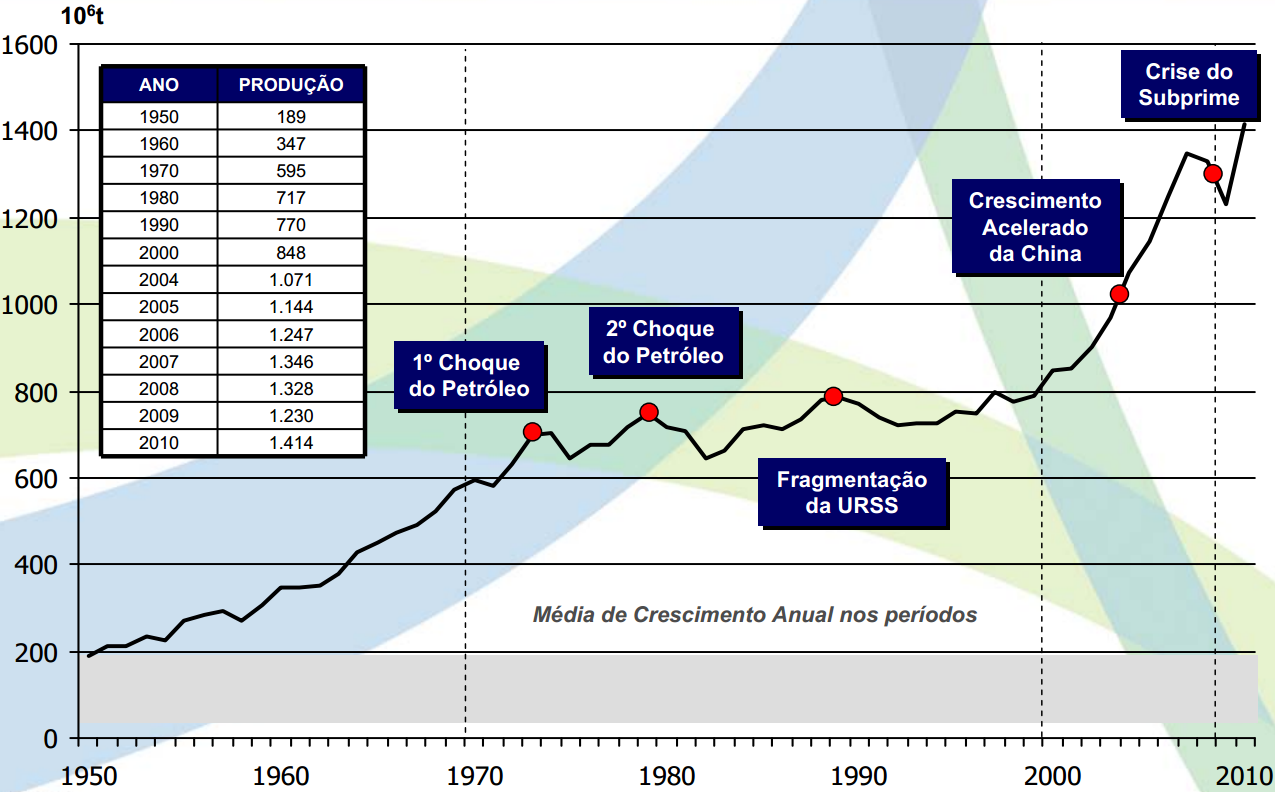
\includegraphics[height=248pt,width=400pt]{images/fig2-1}
    %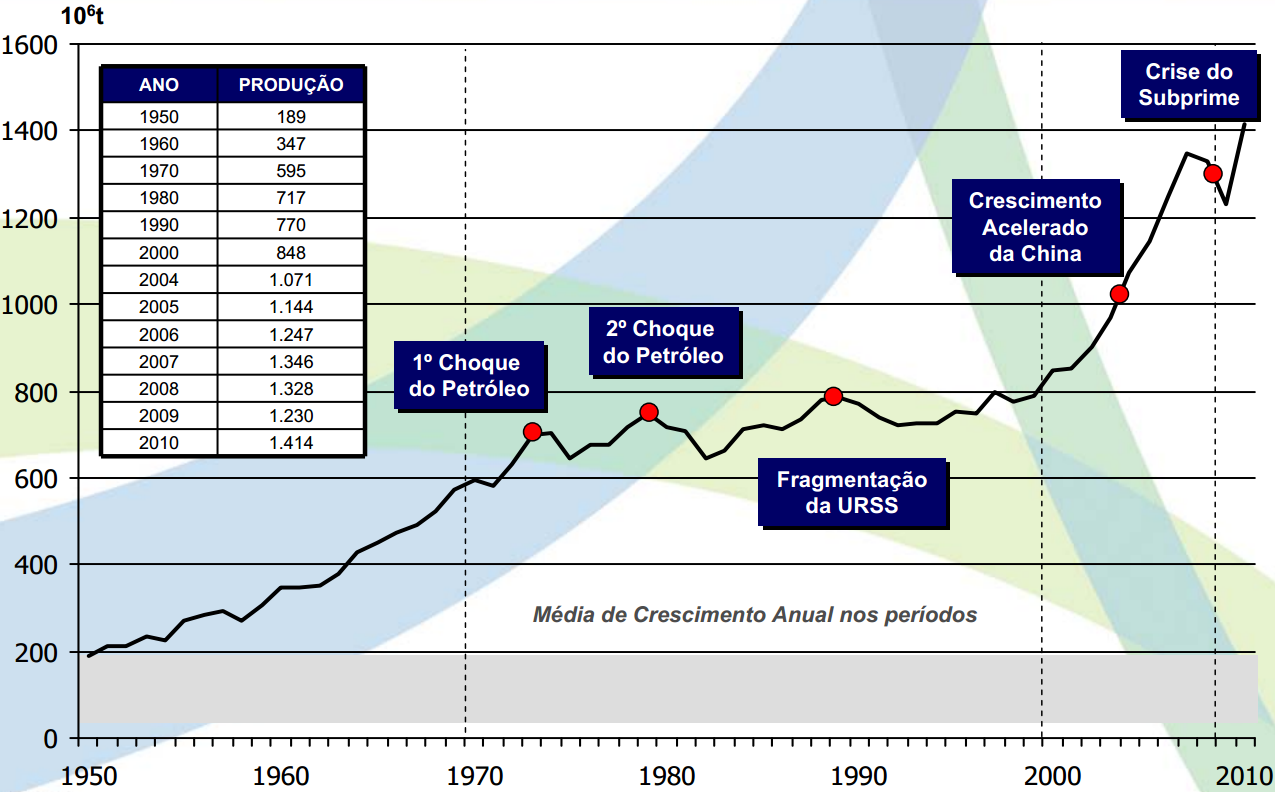
\includegraphics[scale=0.2]{images/fig2-1}
    \caption{Evolução da Produção Mundial de Aço Bruto no período 1950
      - 2010.\cite{24}}\label{fig:2-1}
  \end{center}
\end{figure}
 
A dependência chinesa de recursos naturais externos é de fato a
principal barreira a seu crescimento no longo prazo, e o Brasil
representa uma fonte segura de abastecimento aos chineses nas próximas
décadas. Segundo dados do Conselho Empresarial Brasil-China, entre
1989 e 2004 a China foi responsável por 56\% do crescimento do consumo
de minério de ferro em todo o mundo. Em 2010, a China importou quase
60\% das exportações mundiais de minério de ferro total e produziu
cerca de 60\% de ferro gusa do mundo.\cite{25}

O Brasil é o segundo maior produtor de minério de ferro, conforme a
Conferência das Nações Unidas para o Comércio e o Desenvolvimento
(\uppercase{Unctad}).  Em 2010, o país produziu 372 milhões de
toneladas, o que corresponde a 15,5\% da produção mundial
(Tabela~\ref{tab:2-3}).\cite{20} As vantagens das abundantes reservas
brasileiras devem-se a suas características naturais, cujas jazidas
são de ótima qualidade e de fácil extração, produzindo grandes volumes
a baixos custos.

% -*- coding: utf-8; -*-

\begin{table} [!h]
 \begin{center}  \footnotesize
  \caption{Produção Mineral (em milhões de tons/ano).\cite{20}} \label{tab:2-3}
  ~\\[-1mm]
   \begin{tabularx}
     {\textwidth}
     { % >{\color{blue}}
       p{1.1cm}
       @{}n{4}{1}
       @{\extracolsep{2mm}}n{4}{1}
       @{\extracolsep{2mm}}n{4}{1}
       @{\extracolsep{2mm}}n{4}{1}
       @{\extracolsep{2mm}}n{4}{1}
       @{\extracolsep{2mm}}n{4}{1}
       @{\extracolsep{2mm}}n{4}{1}
       @{\extracolsep{2mm}}n{4}{1}
       @{\extracolsep{2mm}}n{4}{1}
       @{\extracolsep{2mm}}n{4}{1}
       @{\extracolsep{2mm}}n{4}{1}
       @{\extracolsep{2mm}}n{4}{1}
       @{\extracolsep{2mm}}n{4}{1} }
%     { p{2.5cm}
%       @{\extracolsep{.4mm}} C
%       @{\extracolsep{1.0mm}} C
%       @{\extracolsep{1.0mm}} C
%       @{\extracolsep{1.0mm}} C
%       @{\extracolsep{1.0mm}} C
%       @{\extracolsep{1.0mm}} C
%       @{\extracolsep{1.0mm}} C
%       @{\extracolsep{1.0mm}} C
%       @{\extracolsep{1.0mm}} C
%       @{\extracolsep{1.0mm}} C
%       @{\extracolsep{1.0mm}} C}

   \textbf{Ano}
   & \textbf{2000}
   & \textbf{2001}
   & \textbf{2002}
   & \textbf{2003}
   & \textbf{2004}
   & \textbf{2005}
   & \textbf{2006}
   & \textbf{2007}
   & \textbf{2008}
   & \textbf{2009}
   & \textbf{2010} \\ \toprule

   ~\\[-2mm]
   %\rowcolor{Gainsboro}
   PM$^\dag$
   % \begin{tabular}{l}
   %  %\rowcolor{Gainsboro}
   %  Produção\\Mundial
   %\end{tabular}
   & 1060
   & 1060
   & 1080
   & 1060
   & 1340
   & 1540
   & 1712
   & 1900
   & 2200
   & 2240
   & 2400 \\ \midrule

   PB
   %\begin{tabular}{l}
   %  Produção\\Brasil
   %\end{tabular}
   & 212
   & 237
   & 214
   & 264
   & 262
   & 278
   & 317
   & 350
   & 351
   & 331
   & 372 \\ \midrule


   %\rowcolor{Gainsboro}
   PB {\scriptsize [\%]}
   %\begin{tabular}{l}
   %  %\rowcolor{Gainsboro}
   %  \multirow{2}{*}{\% Brasil}\\~
   %\end{tabular}
   & 20.0
   & 22.0
   & 19.8
   & 22.7
   & 19.5
   & 18.0
   & 18.5
   & 18.4
   & 15.9
   & 14.8
   & 15.5 \\ \midrule

   CM
   %\begin{tabular}{l}
   %  Colocação\\Mundial
   %\end{tabular}
   %& \multicolumn{11}{c}{permaneceu no segundo lugar desde 2000}
    & \colmund{2} & \colmund{2} & \colmund{2} & \colmund{2} & \colmund{2}
    & \colmund{2} & \colmund{2} & \colmund{2} & \colmund{2} & \colmund{2} & \colmund{2}
   \\ \midrule

   EB
   % \rowcolor{Gainsboro}
   %\begin{tabular}{l}
   % %\rowcolor{Gainsboro}
   % Exportação\\
   % Brasil
   %\end{tabular}
   & 157
   & 156
   & 167
   & 175
   & 211
   & 224
   & 242
   & 269
   & 282
   & 266
   & 311 \\ \midrule

   EB {\scriptsize [\%]}
   % \begin{tabular}{l}
   %  \multirow{2}{*}{
   %  \% Exportação} \\~
   %  %\% Export.} \\~
   %\end{tabular}
   & 74.0
   & 65.8
   & 78.0
   & 66.3
   & 80.5
   & 80.6
   & 76.3
   & 76.8
   & 80.3
   & 80.4
   & 83.6 \\

  \end{tabularx}
 \end{center}
{$^\dag$ \scriptsize PM: Produção Mundial; PB: Produção Brasileira; CM: Colocação Mundial; EB: Exportação Brasileira}
\end{table}

Os minérios brasileiros apresentam texturas muito variadas, devido às
diferentes condições de metamorfismo, tectonismo e intemperismo a que
foram sujeitos, ou, mesmo, em virtude de sua gênese. Consequentemente,
dentro de uma mesma amostragem, poderão ocorrer minérios de diferentes
características mineralógicas e microestruturais.\cite{10,26,27}

O ferro é encontrado em diversos minerais, mas apenas alguns são
economicamente viáveis como fontes deste elemento, sendo os óxidos os
mais importantes.\cite{28,29} Os principais tipos de texturas de
óxidos e hidróxidos de ferro e suas características são apresentadas
na Tabela~\ref{tab:2-5}.\cite{14}

%% -*- coding: utf-8; -*-

\begin{table} [!h]
  \caption{Principais minerais de ferro e suas classes.\cite{29}}\label{tab:2-4}
  ~\\[-1mm]
   \begin{tabularx}
     {\textwidth}
     { p{2.0cm}
       p{2.5cm}
       p{3.3cm}
       p{1.3cm}
       p{2.7cm}}

     \textbf{Classes}
     & \textbf{Minerais}
     & \textbf{\mrcel {Fórmula}{Química}}
     & \textbf{\mrcel{Teor}{de Fe}}
     & \textbf{\mrcel{~~Designação}{~~Comum}}
     \\\toprule

     ~ \\[-6mm]
     \multirow{5}{*}{Óxidos}& Magnetita
     & $Fe_{3}O_{4}$
     & ~72,4
     & \mrcel{~~Óxido ferroso}{~~férrico}
     \\%\midrule

     & Hematita
     & $Fe_{2}O_{3}$
     & ~69,9
     & ~~Óxido férrico \\[2mm]

     & Goethita
     & $FeO(OH)$
     & ~62,8
     & \multirow{2}{*}{\mrcel{Óxido-hidróxido}{de ferro}} \\[2mm]


     & Lepidocrocita
     & $FeO(OH)$
     & ~62,8 &
     \\\midrule

     Carbonato
     & Siderita
     & $FeCO_{3}$
     & ~48,2
     & \mrcel{~~~~Carbonato}{~~~~de Ferro}
     \\\midrule

     \multirow{2}{*}{Sulfetos}
     & Pirita
     & $FeS_{2}$
     & ~46,5
     & \multirow{2}{*}{~} \\[2mm]


     & Pirrotita
     & $FeS$
     & ~63,6
     & ~
     \\\midrule

     \multirow{10}{*}{Silicatos}
     & Fayalita
     & $Fe^{2+}_{2}(SiO_{4})$
     & ~54,8
     & \mrcel{~~~~Grupo da}{~~~~Olivina} \\[4mm]

     & Laihunite
     & $Fe^{2+}Fe^{3+}_{2}(SiO_{4})_{2}$
     & ~47,6
     & \mrcel{~~~~Grupo da}{~~~~Olivina} \\[4mm]

     & Greenalita
     & \mrcell{$2Fe^{2+}_{2}6Fe^{3+}Si_{2}$}{$4O_{5}(OH)_{3,3}$}
     & ~44,1
     & \mrcel{~~~~Grupo da}{~~~~Serpentina} \\[4mm]

     & Grunerita
     & \mrcell{$Fe^{2+}_{7}(Si_{8}O_{22})$}{$(OH)_{2}$}
     & ~39,0
     & \mrcel{~~~~Grupo dos}{~~~~Anfibólios} \\[4mm]

     & Fé-antofilita
     & \mrcell{$Fe^{2+}_{7}(Si_{8}O_{22})$}{$(OH)_{2}$}
     & ~39,0
     & \mrcel{~~~~Grupo dos}{~~~~Anfibólios}
     \\\midrule
   \end{tabularx}
\end{table}

% -*- coding: utf-8; -*-

\newcommand{\coltworowone}{%
\begin{tabular}{ l @{\extracolsep{2mm}}X }
  \mybulletOB
    & Cristais ~~ muito	\\[-1.2mm]
  ~ & pequenos, 	\\[-.4mm]
  ~ & $<0.01$ mm. \\
  \mybulletOB & Textura porosa. \\
  \mybulletOB
    & Contatos pouco	\\[-1.2mm]
  ~ & desenvolvidos.
\end{tabular}}

\newcommand{\coltworowtwo}{%
\begin{tabular}{ l @{\extracolsep{2mm}}X }
  \mybulletOB
    & Cristais euédricos \\[-1.2mm]
  ~ & isolados ~ ou ~ em \\[-1.2mm]
  ~ & agregados. \\
  \mybulletOB
    & Cristais compac- \\[-1.2mm]
  ~ & tos.
\end{tabular}}

\newcommand{\coltworowthree}{%
\begin{tabular}{ l @{\extracolsep{2mm}}X }
  \mybulletOB
    & Hematita ~~ com \\[-1.2mm]
  ~ & hábito de magne- \\[-1.2mm]
  ~ & tita. \\
  \mybulletOB
    & Oxidação segundo \\[-1.2mm]
  ~ & os planos ~ crista- \\[-1.2mm]
  ~ & lográficos da mag- \\[-1.2mm]
  ~ & netita. \\
  \mybulletOB
    & Geralmente ~ po- \\[-1.6mm]
  ~ & rosa.
\end{tabular}}

\newcommand{\coltworowfour}{%
\begin{tabular}{ l @{\extracolsep{2mm}}X }
  \mybulletOB
    & Formatos irregu- \\[-1.2mm]
  ~ & lares ~~ inequidi- \\[-1.2mm]
  ~ & mensionais. \\
  \mybulletOB
    & Contatos irregula-\\[-1.2mm]
  ~ & res, ~ geralmente \\[-1.2mm]
  ~ & imbricados.
 \end{tabular}}

\newcommand{\coltworowfive}{%
\begin{tabular}{ l @{\extracolsep{2mm}}X }
  \mybulletOB
    & Formatos regula- \\[-1.2mm]
  ~ & res ~~ equidimen- \\[-1.2mm]
  ~ & sionais. \\
  \mybulletOB
    & Contatos ~~ retilí- \\[-1.2mm]
  ~ & neos ~ e ~ junções \\[-1.2mm]
  ~ & tríplices. \\
  \mybulletOB
    & Cristais compac-\\[-1.6mm]
  ~ & tos.
 \end{tabular}}

\newcommand{\coltworowsix}{%
\begin{tabular}{ l @{\extracolsep{2mm}}X }
  \mybulletOB
    & Cristais inequidi- \\[-1.2mm]
  ~ & mensionais, hábi- \\[-1.2mm]
  ~ & to tabular. \\
  \mybulletOB
    & Contato retilíneo. \\
  \mybulletOB
    & Cristais compac- \\[-1.6mm]
  ~ & tos.
 \end{tabular}}

\newcommand{\coltworowseven}{%
\begin{tabular}{ l @{\extracolsep{2mm}}X }
  \mybulletOB
    & Material cripto- \\[-1.2mm]
  ~ & cristalino.  \\
  \mybulletOB
    & Estrutura colofor- \\[-1.2mm]
  ~ & me, hábito botri- \\[-1.2mm]
  ~ & oidal.  \\
  \mybulletOB
    & Textura porosa.
 \end{tabular}}

\begin{table} [!p]
    \caption{Main morphologies of hematite.\cite{14}}\label{tab:2-5}
    ~\\[-2mm]
  \begin{tabularx}{\textwidth}{@{\extracolsep{0pt}}C @{\extracolsep{0pt}}C C C}

    \textbf{Tipo}
    & \textbf{Características}
    & \textbf{\mrcel{Forma}{Textura}}
    & \textbf{\mrcel{Ilustração}{Esquemática}}
    \\\toprule

    ~ \\[-6mm]
    \mrcel{Hematita}{Microcristalina}
    & \coltworowone
    & \mytbcimg{2.3cm}{2.9cm}{images/Microcristalina}
    & \mytbcimg{2.6cm}{2.5cm}{images/MicrocristalinaEsq}
    \\\midrule

    ~\\[-6mm]
    Magnetita
    & \coltworowtwo
    & \mytbcimg{2.3cm}{2.9cm}{images/Magnetita}
    & \mytbcimg{2.6cm}{2.9cm}{images/MagnetitaEsq}
    \\\midrule

    ~\\[-5mm]
    Martita
    & \coltworowthree
    & \mytbcimg{2.3cm}{2.9cm}{images/Martita}
    & \mytbcimg{2.6cm}{2.9cm}{images/MartitaEsq}
    \\\midrule

    ~\\[-5mm]
    \mrcel{Hematita}{Lobular}
    & \coltworowfour
    & \mytbcimg{2.3cm}{2.9cm}{images/Lobular}
    & \mytbcimg{2.6cm}{2.9cm}{images/LobularEsq}
    \\\midrule

    ~\\[-5mm]
    \mrcel{Hematita}{Granular}
    & \coltworowfive
    & \mytbcimg{2.3cm}{2.9cm}{images/Granular}
    & \mytbcimg{2.6cm}{2.9cm}{images/GranularEsq}
    \\\midrule

    ~\\[-5mm]
    \mrcel{Hematita}{Lamelar}
    & \coltworowsix
    & \mytbcimg{2.3cm}{2.9cm}{images/Lamelar}
    & \mytbcimg{2.6cm}{2.9cm}{images/LamelarEsq}
    \\\midrule

    ~\\[-5mm]
    \mrcelthree{Hidróxidos de}{ Fe (Goethita-}{Limonita)}
    & \coltworowseven
    & \mytbcimg{2.3cm}{2.9cm}{images/Goethita}
    & \mytbcimg{2.6cm}{2.9cm}{images/GoethitaEsq}
    \\\midrule

  \end{tabularx}
\end{table}


\subsection{Hematita}

A hematita é o mineral de ferro mais importante devido a sua alta
ocorrência em vários tipos de rochas e suas origens diversas.\cite{30}
A composição química deste mineral é Fe$_{2}$O$_{3}$, com uma fração
mássica em ferro de 69,9\% e uma fração mássica em oxigênio de
30,1\%.\cite{31}

Este mineral pode ser encontrado com diferentes morfologias
(Tabela~\ref{tab:2-5}), como, por exemplo, microcristalina, lobular,
granular ou lamelar. A hematita também pode ser encontrada com hábito
de magnetita formando uma fase mista chamada de martita.\cite{2,14}
Estas morfologias estão relacionadas a uma condição de cristalização
diferenciada, que poderá ter influência no seu processamento.\cite{26}

O nome hematita vem do grego \textit{haima} que significa sangue. Como
pode ser observado na Figura~\ref{fig:2-2}a e Figura~\ref{fig:2-2}b a
cor da hematita varia do vermelho-sangue até o preto com forte brilho
metálico. Por sua vez, na Figura~\ref{fig:2-2}c, pode ser observado
que seu arranjo atômico é trigonal-hexagonal (\={3}2/m), com
parâmetros de $a = 5,034$ \AA~e de $c = 13,752$ \AA~e grupo espacial
R\={3}c.\cite{4,31} Esta estrutura hexagonal pode ser observada
facilmente no mineral como mostra a Figura~\ref{fig:2-2}b.

\begin{figure} [h]
  \begin{center}
    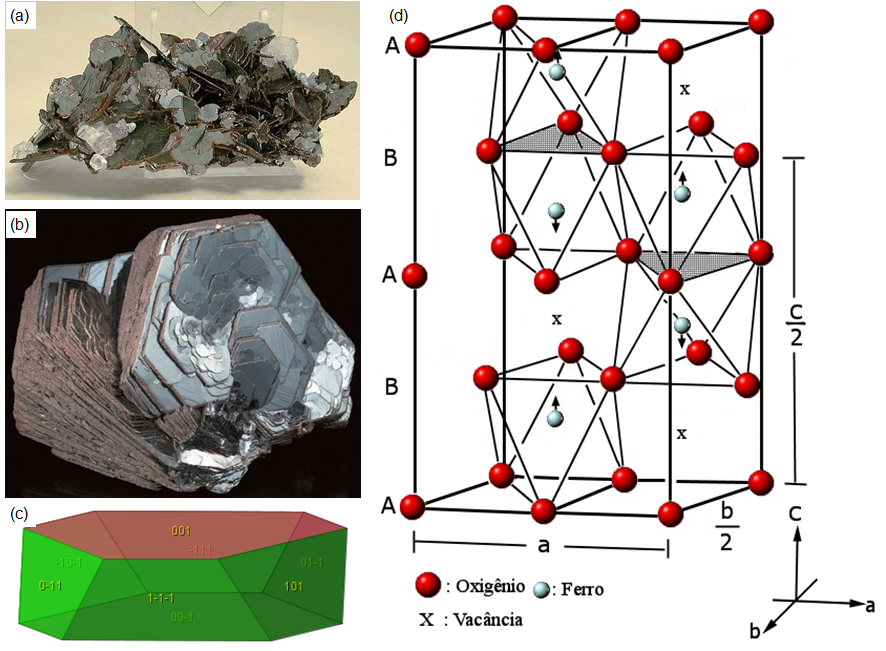
\includegraphics[height=294pt,width=400pt]{images/fig2-2}
    \caption{Hematita: (a) e (b) Imagens de fragmentos do mineral; (c)
      Estrutura trigonal-hexagonal visualizando os planos; (d) Modelo
      de bolas e varetas da cela unitária.\cite{4,31}}\label{fig:2-2}
  \end{center}
\end{figure}

A hematita também pode ser indexada no sistema romboédrico, cuja cela
unitária seria $a_{tr} = 5,427$ \AA~e $\alpha = 55,3\degree$, de tal
forma que existem camadas de oxigênio rodeando átomos de ferro
formando octaedros ligados pelas faces, conforme mostrado na
Figura~\ref{fig:2-2}d. Esta estrutura consiste de um empacotamento
denso de planos de oxigênio empilhados na repetição \textit{ABAB} ao
longo da direção $[001]$ (planos de íons paralelos ao plano (001)) com
os átomos de \textit{Fe} ocupando as posições octaédricas. Dois terços
dos sítios octaedrais estão ocupados por íons $Fe ^{3+}$ que são
arranjados regularmente com dois sítios preenchidos seguidos por um
sítio vacante na direção $[001]$ formando anéis sêxtuplos.\cite{4,32}

O arranjo de cátions produz pares de octaedros $Fe(O)_{6}$. Cada
octaedro compartilha uma face com um octaedro da camada
adjacente. Assim, a estrutura real de hematita é distorcida devido à
repulsão dos átomos de Fe presentes nos octaedros que partilham a
face. Os átomos de Fe, então, se situam mais próximos das faces não
partilhadas (Figura~\ref{fig:2-2}d). A estrutura tripla $Fe-O_{3}-Fe$
influencia as propriedades magnéticas da hematita que, diferente da
magnetita, é um óxido fracamente ferromagnético à temperatura
ambiente.\cite{4,33}

Existem relacionamentos estruturais entre certos planos na estrutura
da hematita e planos em outros óxidos de ferro, especialmente com a
magnetita e a goethita (Tabela~\ref{tab:2-6}). Há, por exemplo, um
relacionamento entre o plano (111) da magnetita e o plano (001) da
hematita. Com isso algumas vezes pode-se observar nucleação e
crescimento de magnetita no plano (001) da hematita. Do mesmo modo,
como resultado da afinidade estrutural entre os planos (100) da
goethita e o plano (003) da hematita, pode ocorrer um crescimento
epitaxial de goethita na hematita.\cite{4}

% -*- coding: utf-8; -*-

\begin{table} [!h]
  \caption{Orientações estruturais entre os óxidos de ferro.\cite{4}}\label{tab:2-6}
  ~\\[-1mm]
   \begin{tabularx}
     {\textwidth}
     { p{2.9cm}
       p{2.7cm}
       p{3.6cm}
       p{3cm}}

     \textbf{\mrcel {Par de}{Óxidos}}
     & \textbf{\mrcel {Fórmula}{Química}}
     & \textbf{\mrcel {Plano}{Cristalográfico}}
     & \textbf{\mrcel {Direção}{Cristalográfica}}
     \\\toprule

     ~ \\[-6mm]
     Goethita
     & $FeO(OH)$
     & (100)(004)(200)
     & [100]
     \\

     Hematita
     & $\alpha-Fe_{2}O_{3}$
     & (003)(110)(100)
     & [100] \\[3mm]
     
     Hematita
     & $\alpha-Fe_{2}O_{3}$
     & (001)
     & [100] \\     

     Magnetita
     & $Fe_{3}O_{4}$
     & (111)
     & [110] \\[3mm]

     Lepidocrocita
     & $FeO(OH)$
     & (100) 
     & [001][051] \\
     
     Maghemita
     & $\gamma-Fe_{2}O_{3}$
     & (001) 
     & [110][111]     
     \\\midrule

   \end{tabularx}
\end{table}


A hematita é um material opaco no MLR, porém em lamelas muito finas e
em luz transmitida é vermelha sanguínea escura, e pode apresentar
dicroísmo de vermelho acastanhado a vermelho amarelado. Este mineral
tem um coeficiente de reflexão médio de 25\%-32\% no ar.\cite{34}
Contudo, a propriedade ótica mais importante deste mineral para o
presente trabalho é sua birrefletância devido à forte anisotropia que
ele apresenta. Assim, sua reflexão e, consequentemente, o seu brilho
na imagem mudam com diferentes orientações dos cristais com relação ao
plano de incidência da luz.\cite{5} Este efeito ainda pode ser
ampliado quando é usada luz polarizada no MLR.

\section{Microscopia Digital}

Podemos definir a MD como a integração entre o microscópio e o
computador, oferecendo automação do microscópio, aquisição e análise
digital de imagens. Esta área, além de permitir a automação, fornece
novos recursos para a caracterização microestrutural.\cite{35}

Alguns sistemas totalmente controlados por software e com ambiente de
programação permitem uma automação completa.\cite{36} Exemplos disto
são:

\begin{enumerate}[label=$\triangleright$]
  \item Uso de rotinas para o controle da platina motorizada;\cite{37}
  \item Troca de lentes;
  \item Correção de defeitos na aquisição;\cite{38,39}
  \item Autofoco;\cite{40,41}
  \item Foco estendido;\cite{42,43}
  \item Ajuste automático da iluminação e cor;\cite{44,45}
  \item Controle dos filtros e dos diafragmas;
  \item Varredura da amostra com aquisição automática de imagens e;
  \item Obtenção de mosaico ou campo estendido.\cite{46}
\end{enumerate}

Algumas destas rotinas vêm incluídas em softwares comerciais de
aquisição e análise de imagens, como o KS400, o AxioVision e o SIS,
apenas para nomear alguns.\cite{47,48,49} O Laboratório de MD da
PUC-Rio (LMD) conta com dois microscópios óticos motorizados, Zeiss
~AxioPlan 2 ~e ~Zeiss AxioImager.M2m, com câmeras digitais, Zeiss
AxioCam HRc e Zeiss AxioCam MRc5 respectivamente, automatizados com o
software AxioVision.\cite{50}

O desenvolvimento de câmeras coloridas CCD (\textit{Charge-Coupled
  Device}) e a integração do controle por computador do conjunto
câmera/microscópio, facilitou a aquisição automática de
imagens.\cite{35,51} Entenda-se por aquisição automática de imagem uma
rotina que faz uma varredura da amostra, capturando imagens de campos
adjacentes ou espaçados, de forma automática. Esse tipo de rotina foi
implementada em softwares comerciais de aquisição e análise de
imagens. Além da maior velocidade e praticidade, o método automático é
reprodutível e evita a ocorrência de erros por fadiga do operador,
como a repetição e a sobreposição de campos.\cite{52}

A MD, além de permitir certo grau de automação, abriu novas
possibilidades para a caracterização microestrutural.\cite{35}

Várias técnicas quantitativas já vinham sendo utilizadas na
caracterização de amostras de minério de ferro.\cite{11} Entre estas
técnicas encontra-se a difratometria de raios X, a espectroscopia
Mössbauer, a análise de imagens obtidas tanto por microscopia ótica
como eletrônica, entre
outras.\cite{6,7,8,32,53,54,55,56,57,58,59,500,501}

A microscopia ótica de luz transmitida, para minerais transparentes, e
de luz refletida, para minerais opacos, é provavelmente o método mais
tradicional de identificação mineralógica.\cite{60} Esta técnica é uma
ferramenta adequada, uma vez que permite obter dados sobre a
porosidade, associações minerais, liberação mineral, forma das
partículas, distribuição por tamanho e textura, entre outras.\cite{30}

Recentemente, alguns autores aplicaram uma técnica de análise de
textura em imagens adquiridas com luz polarizada para classificar
fases de minério de ferro.\cite{58} Embora com algumas limitações, a
metodologia desenvolvida por eles foi promissora na identificação de
cristais de hematita. Esta metodologia se baseia no processamento de
imagens para determinar fronteiras de cristais de hematita onde um
conjunto de sete imagens, por campo, é adquirido girando o polarizador
em pequenos intervalos angulares.

Outros autores também fizeram uso da luz polarizada na identificação e
análise de minerais e rochas.\cite{30,61,62,63,64} É de particular
importância o fato de que este tipo de iluminação produz contraste
entre cristais com orientações diferentes no espaço. Isto possibilita
a visualização dos cristais, geralmente impossíveis de serem vistos
com iluminação convencional em campo claro (Figura~\ref{fig:bf-pol}).

\begin{figure} [h]
  \begin{center}
    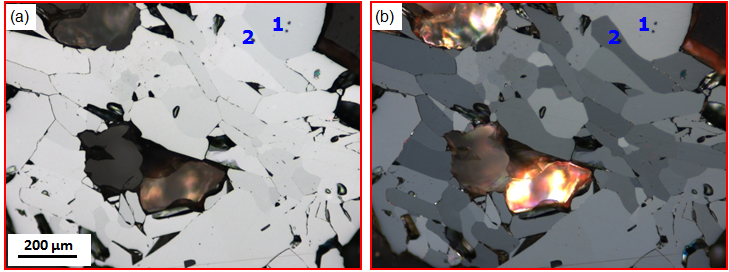
\includegraphics[height=150pt,width=400pt]{images/fig_bf-pol}
    \caption{Variação de brilho entre dois cristais adjacentes: (a)
      Imagem em campo claro; (b) Imagem com polarização de um mesmo
      campo.\cite{65}}\label{fig:bf-pol}
  \end{center}
\end{figure}

A Figura~\ref{fig:bf-pol} mostra duas imagens de um mesmo campo de uma
amostra de minério de ferro adquiridas no MLR, a primeira em campo
claro (Figura~\ref{fig:bf-pol}a) e a segunda sob luz polarizada
(Figura~\ref{fig:bf-pol}b). Na imagem sem polarização dois cristais
adjacentes são indicados, em azul, como 1 e 2.  Neste caso quase não
pode ser observada uma diferença de brilho, embora na imagem com
polarização a diferença de brilho entre esses mesmos cristais seja
muito alta. Assim, fica evidente a importância da luz polarizada, no
âmbito da microscopia ótica da luz refletida, para identificar
cristais de hematita em minérios de ferro.

\subsection{Polarização da Luz}

A luz pode ser tratada como uma onda eletromagnética transversal, ou
seja, os vetores intensidade do campo elétrico ($\vec{E}$) e
intensidade do campo magnético ($\vec{H}$) são ortogonais entre si. A
luz vibra não só num plano, mas em todos os planos simultaneamente,
portanto há planos de ondas em todos os ângulos
(Figura~\ref{fig:luz-nat}). Este tipo de luz é conhecida como luz
natural ou luz não polarizada.\cite{66}

\begin{figure} [h]
  \begin{center}
    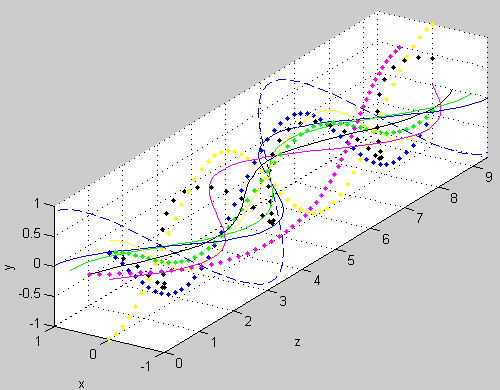
\includegraphics[height=273pt,width=350pt]{images/fig_luz-nat}
    \caption{Luz natural com os diferentes comprimentos de onda
      correspondentes a cada cor. Neste caso só foi representada a
      intensidade do campo elétrico para facilitar a
      visualização.\cite{67}}\label{fig:luz-nat}
  \end{center}
\end{figure}
 
A luz polarizada, diferente da luz natural, vibra num plano só (plano
de polarização) e o os vetores $\vec{E}$ e $\vec{H}$ são normais à
direção de propagação como mostra a Figura~\ref{fig:luz-lpol}. Isto
pode ser demostrado através das equações de Maxwell onde, após algumas
considerações e simplificações, pode-se chegar às seguintes equações
de ondas:

\begin{align}
 &\nabla^2 \vec{E}  = \mu_{0}\epsilon_{0}\frac{\partial^2}{\partial t^{2}}\vec{E}\label{eq-incampele}\\
 &\nabla^2 \vec{H}  = \mu_{0}\epsilon_{0}\frac{\partial^2}{\partial t^{2}}\vec{H}\label{eq-incampmag}
\end{align}

sendo que $\mu_{0}$ é a permeabilidade magnética do vácuo e
$\epsilon_{0}$ a permeabilidade elétrica do vácuo.

\begin{figure} [h]
  \begin{center}
    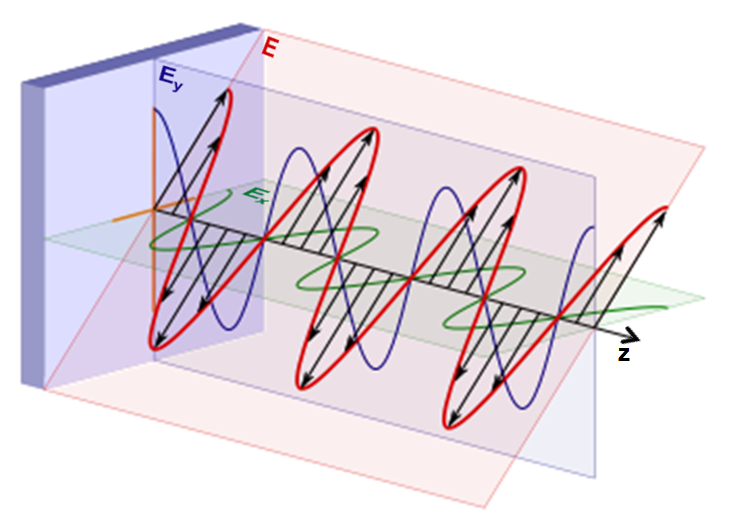
\includegraphics[height=253pt,width=350pt]{images/fig_luz-lpol}
    \caption{Propagação de uma onda plana linearmente
      polarizada. Neste caso só foi representada a intensidade do
      campo elétrico para facilitar a
      visualização.\cite{68}}\label{fig:luz-lpol}
  \end{center}
\end{figure}

As soluções das equações \eqref{eq-incampele} e \eqref{eq-incampmag}
seriam:

\begin{align}
 &\vec{E}  = \vec{E}_{x} + \vec{E}_{y} \\
 &\vec{H}  = \vec{H}_{x} + \vec{H}_{y} \\
 &\vec{E}  = E_{0x}\hat{x}\exp[i(\vec{k}\vec{z}-wt)] + E_{0y}\hat{y}\exp[i(\vec{k}\vec{z}-wt)]\\
 &\vec{H}  = H_{0x}\hat{x}\exp[i(\vec{k}\vec{z}-wt)] + H_{0y}\hat{y}\exp[i(\vec{k}\vec{z}-wt)]\\
 &\vec{E}  = (E_{0x}\hat{x} + E_{0y}\hat{y})\exp[i(\vec{k}\vec{z}-wt)]
\end{align}

tomando a parte real do vetor, temos que:

\begin{align}
 &\vec{E}  = (E_{0x}\hat{x} + E_{0y}\hat{y})\cos(\vec{k}\vec{z}-wt)\label{eq-ellpol}\\
 &\vec{E}  = \vec{E}_{0}\cos(\vec{k}\vec{z}-wt)\label{eq-ellpol}\\
 &\vec{H}  = (H_{0x}\hat{x} + H_{0y}\hat{y})\cos(\vec{k}\vec{z}-wt)\label{eq-hllpol}\\
 &\vec{H}  = \vec{H}_{0}\cos(\vec{k}\vec{z}-wt)\label{eq-ellpol}
\end{align}

onde $\frac{w}{k}=c=\frac{1}{\sqrt{\mu_{0}\epsilon_{0}}}$ ($c$ é a
velocidade da luz no vácuo, $k$ o módulo do vetor de onda, $w$ a
frequência e $t$ o tempo). Portanto, a onda resultante tem uma
amplitude fixa igual a $\vec{E}_{0} = E_{0x}\hat{x} + E_{0y}\hat{y}$
para a intensidade do campo elétrico e $\vec{H}_{0} = H_{0x}\hat{x} +
H_{0y}\hat{y}$ para a intensidade do campo magnético ou seja, ela
também é linearmente polarizada. Assim, a onda resultante $\vec{E}$ (e
consequentemente $\vec{H}$) oscila ao longo de um plano inclinado,
como mostra a Figura~\ref{fig:luz-lpol}, segundo uma cossenoide no
tempo.

A luz, além de ser linearmente polarizada, também pode ser circular e
elipticamente polarizada. A polarização circular é um caso particular
da polarização elíptica porém, esta última, não será detalhada por não
ter sido utilizada neste trabalho.

No caso da polarização linear, a projeção do vetor $\vec{E}$ sobre o
plano $xy$ descreve um segmento de reta. No entanto, quando ambas
ondas constitutivas têm a mesma amplitude (ou seja, $E_{0x}$ =
$E_{0y}$ = $E_{0}$ e consequentemente $H_{0x}$ = $H_{0y}$ = $H_{0}$) a
projeção será uma circunferência. Neste tipo de polarização, a soma de
dois campos $\vec{E}_{x}$ e $\vec{E}_{y}$ (e consequentemente de
$\vec{H}_{x}$ e $\vec{H}_{y}$) se propaga na direção $z$ com a mesma
frequência e vetor de onda, porém com uma desfasagem de $\phi$=$\pi/2$
(Figura~\ref{fig:luz-cpol}).

\begin{figure} [h]
  \begin{center}
    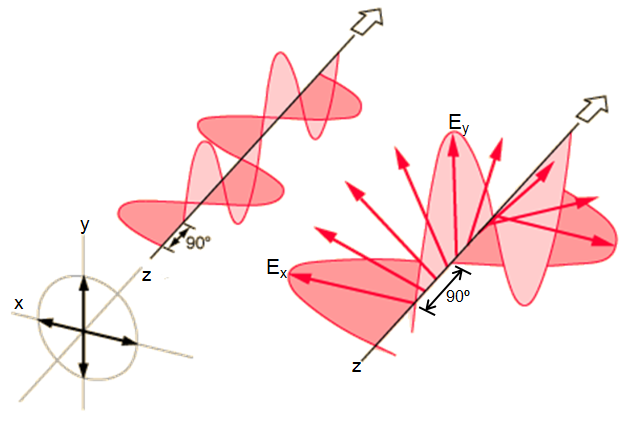
\includegraphics[height=235pt,width=350pt]{images/fig_luz-cpol}
    \caption{Propagação de uma onda com polarização circular. Neste
      caso só foi representada a intensidade do campo elétrico para
      facilitar a visualização.\cite{69}}\label{fig:luz-cpol}
  \end{center}
 \end{figure}

 Neste caso, a solução das equações \eqref{eq-incampele} e
 \eqref{eq-incampmag} seria:

\begin{align}
 &~~~~~~\vec{E}  = \vec{E}_{x} + \vec{E}_{y} \\
 &~~~~~~\vec{H}  = \vec{H}_{x} + \vec{H}_{y} \\
 &~~~~~~\vec{E}  = E_{0}\hat{x}\exp[i(\vec{k}\vec{z}-wt)] + E_{0}\hat{y}\exp[i(\vec{k}\vec{z}-wt+\pi/2)]\\
 &~~~~~~\vec{H}  = H_{0}\hat{x}\exp[i(\vec{k}\vec{z}-wt)] + H_{0}\hat{y}\exp[i(\vec{k}\vec{z}-wt+\pi/2)]
\end{align}

tomando a parte real do vetor, temos que:

\begin{align}
 &\vec{E} = E_{0}\hat{x}\cos(\vec{k}\vec{z}-wt) + E_{0}\hat{y}\cos(\vec{k}\vec{z}-wt+\pi/2)\\
 &\vec{H} = H_{0}\hat{x}\cos(\vec{k}\vec{z}-wt) + H_{0}\hat{y}\cos(\vec{k}\vec{z}-wt+\pi/2)\\
 &\vec{E} = E_{0}\hat{x}\cos(\vec{k}\vec{z}-wt) + E_{0}\hat{y}\sin(\vec{k}\vec{z}-wt) \label{eq-ec}\\
 &\vec{H} = H_{0}\hat{x}\cos(\vec{k}\vec{z}-wt) + H_{0}\hat{y}\sin(\vec{k}\vec{z}-wt) \label{eq-hc}\\
 &\vec{E}_{x} = E_{0}\hat{x}\cos(\vec{k}\vec{z}-wt)\label{eq-ex}\\
 &\vec{H}_{x} = H_{0}\hat{x}\cos(\vec{k}\vec{z}-wt)\label{eq-hx}\\
 &\vec{E}_{y} = E_{0}\hat{y}\sin(\vec{k}\vec{z}-wt)\label{eq-ey}\\
 &\vec{H}_{y} = H_{0}\hat{y}\sin(\vec{k}\vec{z}-wt)\label{eq-hy}\\
 &\|\vec{E}\| =\sqrt{(\vec{E}_{x})^2+(\vec{E}_{y})^2} = E_{0}\label{eq-er}\\
 &\|\vec{H}\| =\sqrt{(\vec{H}_{x})^2+(\vec{H}_{y})^2} = H_{0}\label{eq-hr}
\end{align}

onde $\hat{x}$ e $\hat{y}$ são os vetores unitários na direção $x$ e
$y$, respectivamente. Pode-se observar que as amplitudes escalares de
$\vec{E}$ e $\vec{H}$ são contantes. Contudo, as direções dos vetores
variam no espaço e tempo, girando no sentido horário, e sua projeção
no plano $xy$ descreve uma circunferência (Figura~\ref{fig:luz-cpol}).

Microscópios com polarização são poderosos instrumentos analíticos em
estudos petrográficos e análise de minérios.\cite{50} Quando um
mineral anisotrópico, composto por cristais com orientações
diferentes, é observado ao microscópio de luz polarizada, se faz
visível a diferença de brilho ente os cristais.

Os microscópios com polarização linear são dotados de dois
polarizadores designados de polarizador e analisador. Nos microscópios
modernos, estes polarizadores são constituídos de placas de
polaróides. Um polaróide é formado por um composto químico orgânico
(álcool polivinílico) embebido em iodo e estirado segundo uma certa
direção. Desta forma as longas moléculas do material são alinhadas,
assim o iodo se liga às cadeias alongadas das moléculas
poliméricas. Deste modo, os eléctrons dos íons de iodo podem
deslocar-se ao longo das cadeias moleculares, tal como num fio
condutor.

A componente do campo $\vec{E}$, da luz natural incidente, paralela às
moléculas executa trabalho sobre os eléctrons e é absorvida. Assim, o
eixo de transmissão do polaróide é normal à orientação das
moléculas. A luz linearmente polarizada incide na amostra e é
refletida. Um segundo polaróide (o analisador) deixará passar apenas a
componente do campo elétrico que vibra na direção de seu eixo de
transmissão. Desta forma, se $\vec{E}_{0}$ é a intensidade do campo
elétrico determinada pelo polarizador somente sua componente
$\vec{E}_{0}\cos(\theta)$, paralela ao eixo de transmissão do
analisador, passará pelo analisador. Neste caso, $\theta$ é o ângulo
entre os eixos de transmissão do polarizador e o analisador. Um
exemplo de imagem obtida por polarização linear pode ser observada na
Figura~\ref{fig:bf-pol-cpol}b.

\begin{figure} [h]
  \begin{center}
    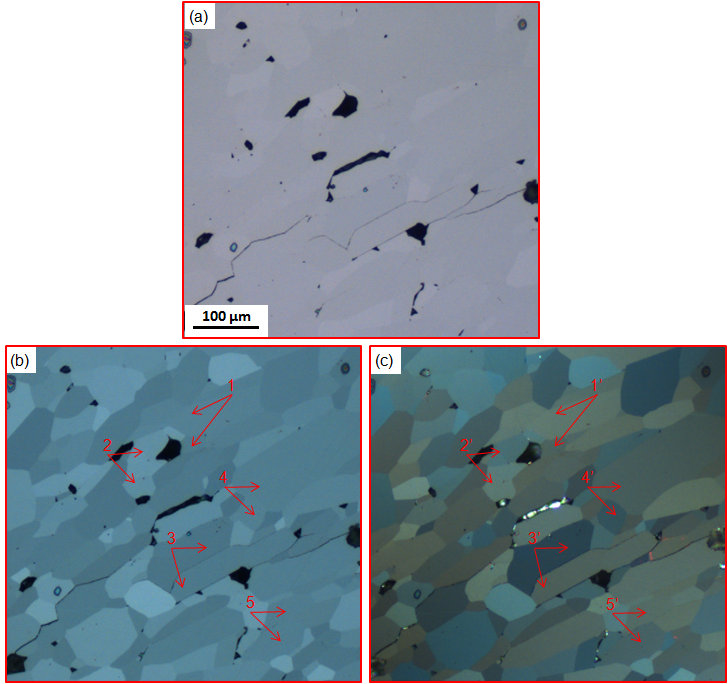
\includegraphics[height=376pt,width=400pt]{images/fig_bf-pol-cpol}
    \caption{Variação de brilho entre cristais adjacentes: (a) Imagem
      em campo claro; (b) Imagem com polarização linear; (c) Imagem
      com polarização circular, de um mesmo
      campo.}\label{fig:bf-pol-cpol}
  \end{center}
\end{figure}
 
Por outro lado, alguns microscópios óticos modernos, além da
polarização linear da luz, permitem também a polarização
circular.\cite{70} O microscópio usado no presente trabalho conta com
um sistema ótico composto por um polarizador, um analisador e duas
placas de um quarto de onda, colocados em um refletor. Ambos os lados
do refletor, entrada e saída de luz, são constituídos por uma
combinação de polarizador e placa de um quarto de onda, fixados
transversalmente.

Deste modo, a luz não-polarizada passa pelo polarizador, tornando-se
linearmente polarizada. Então, a luz linearmente polarizada incide na
primeira placa de um quarto de onda, orientada com um ângulo de 45° em
relação ao plano de polarização da luz incidente. Essa placa divide a
luz em duas componentes com uma diferença de fase de 90°. A combinação
dessas duas ondas linearmente polarizadas, de mesma amplitude e
defasadas de 90°, resulta em uma onda circularmente polarizada, como
mostrado na Figura~\ref{fig:luz-cpol}.\cite{71}

A luz circularmente polarizada incide na amostra e é refletida. Então,
a luz refletida passa pela segunda placa de um quarto de onda, que é
orientada ortogonalmente à primeira. A segunda placa converte a luz
circularmente polarizada em linearmente polarizada, com uma orientação
diferente da do polarizador. Em seguida, essa luz passa pelo
analisador e segue para a câmera.\cite{71}

Na imagem resultante da polarização circular, não há ponto de
extinção, pois todas as orientações de polarização estão
presentes.\cite{71} A polarização circular é uma inovadora técnica em
microscopia de materiais, permitindo melhorar o contraste na
imagem. Além disso, as cores não variam com a rotação da
amostra. Assim, objetos que costumavam ser visíveis apenas em uma
certa direção agora podem ser vistas em sua totalidade
(Figura~\ref{fig:bf-pol-cpol}), independente de sua orientação e sem
rotação da platina.\cite{50}

Na Figura~\ref{fig:bf-pol-cpol} pode-se observar três imagens de um
mesmo campo de uma amostra de minério de ferro, a primeira em campo
claro (Figura~\ref{fig:bf-pol-cpol}a), a segunda com polarização
linear (Figura~\ref{fig:bf-pol-cpol}b) e a terceira com polarização
circular (Figura~\ref{fig:bf-pol-cpol}c). Após observar os pares de
pontos indicados em vermelho (1-1', 2-2', 3-3' e 4-4'), nas
Figuras~\ref{fig:bf-pol-cpol}b e \ref{fig:bf-pol-cpol}c, fica evidente
a superioridade de contraste da luz circularmente polarizada. Cristais
com o mesmo brilho na Figura~\ref{fig:bf-pol-cpol}b foram totalmente
diferençados na Figura~\ref{fig:bf-pol-cpol}c. A formação de contraste
entre os cristais de hematita, por luz polarizada, desempenha um papel
central no método de segmentação de cristais proposto neste trabalho.

\section{Processamento e Análise Digital de Imagens}

O Processamento Digital de Imagens (PDI) é uma técnica que utiliza
operações matemáticas para alterar os valores dos pixels de uma imagem
digital, modificando-a para facilitar sua visualização e análise. Por
sua vez, a Análise Digital de Imagens (ADI) consiste na extração e
tratamento de dados quantitativos de imagens digitais. Deste modo,
utiliza-se o termo Processamento e Análise Digital de Imagens (PADI)
para englobar as duas técnicas anteriores.\cite{72}

A Figura~\ref{fig:2-4} apresenta a sequência padrão de
PADI.\cite{35,52,72,73} Esta sequência está dividida em três blocos
básicos:

\begin{enumerate}[label=(\roman{*})]
  \item A aquisição, que envolve a formação e a digitalização da imagem;
  \item O PDI, no qual encontra-se a etapa de pré-processamento, que
    tem como objetivo melhorar a qualidade da imagem para facilitar
    sua visualização e análise e;
  \item E finalmente a ADI, onde finalmente ocorre a identificação dos
    objetos dos quais são extraídos e tratados os dados
    quantitativos. Neste bloco encontram-se as etapas de segmentação,
    pós-processamento, extração de atributos e reconhecimento e
    classificação.
\end{enumerate}

\begin{figure} [h]
  \begin{center}
    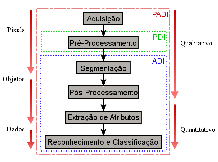
\includegraphics[height=225pt,width=350pt]{images/fig2-4}
    \caption{Sequência padrão de PADI por etapas.\cite{52}}\label{fig:2-4}
  \end{center}
\end{figure}

Nos lados da sequência padrão aparecem setas que indicam o nível
semântico dos dados sobre os quais se trabalha. No pré-processamento e
na segmentação, opera-se diretamente sobre os pixels da imagem,
gerando-se uma imagem com objetos, representados por regiões de pixels
contíguos de mesmo valor. No pós-processamento trabalha-se sobre os
objetos que serão medidos na extração de atributos. A partir daí, na
etapa de reconhecimento e classificação, trabalha-se com estas
medidas, gerando dados de mais alto nível.

Esta sequência padrão tem sido discutida amplamente em trabalhos
prévios do grupo, por isso só as etapas e suas rotinas de interesse
para este trabalho serão abordadas a seguir.\cite{35,52,72,73,74}

\subsection{Pré-processamento}

A etapa de pré-processamento é o primeiro passo depois da aquisição da
imagem. Esta etapa tem como objetivo melhorar a qualidade da imagem,
seja corrigindo defeitos gerados durante a aquisição ou seja realçando
detalhes de interesse específico.

\subsubsection{Registro de imagem}

A primeira coisa a se fazer quando várias imagens de um mesmo campo
são capturadas com diferentes sensores ou com um mesmo sensor, porém
sob diferentes condições de captura, é um registro espacial das
mesmas.\cite{75} O registro é um importante passo, no
pré-processamento, a fim de criar imagens geometricamente iguais com
uma coerência pixel a pixel.

O registro de imagem é normalmente utilizado em sensoriamento remoto,
na medicina, na cartografia, em processamento digital de imagens,
entre outras. Durante as últimas décadas, os dispositivos de aquisição
de imagens passaram por um rápido desenvolvimento. Assim, uma
crescente e diversa quantidade de imagens estavam sendo obtidas,
invocando pesquisas sobre registro automático de imagem.\cite{76}
Existe na literatura uma grande variedade de trabalhos relacionados
com o registro de imagens, baseados em diferentes princípios e com
emprego em diversas aplicações.\cite{75,76,77,78,79,80,81,82,83}

O registro basicamente consiste em corrigir o alinhamento geométrico
de duas ou mais imagens de um mesmo campo. Para isto, toma-se uma
imagem como referência enquanto as outras são registradas a ela. O
registro consiste em encontrar uma transformação capaz de remapear as
posições dos pixels da imagem registrada de modo que a área sobreposta
esteja alinhada com a imagem de referência.\cite{77}

Contudo, a transformação capaz de remapear as posições dos pixels das
duas imagens pode ser bastante complexa. Esta transformação pode ser
composta por uma combinação de transformações de basicamente seis
naturezas distintas:

\begin{enumerate}[label=$\triangleright$]
  \item Translação;
  \item Rotação;
  \item Escala;
  \item Paralelismo;
  \item Projeção e;
  \item Outras distorções como curvas, distorções locais, etc.\cite{52}
\end{enumerate}

A Figura~\ref{fig:posiv-transf} apresenta estas diferentes
transformações, mostrando claramente seu efeito em uma imagem exemplo.

\begin{figure} [h]
  \begin{center}
    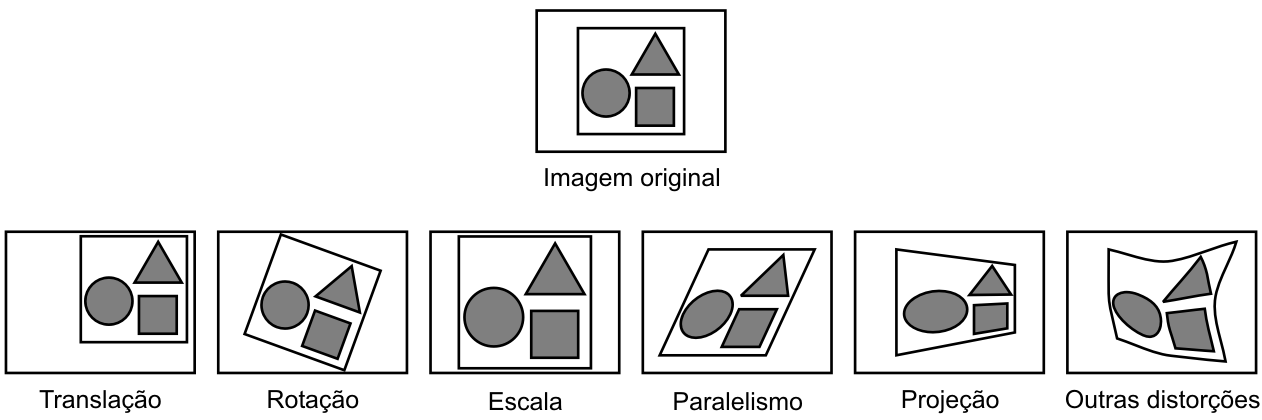
\includegraphics[height=117pt,width=350pt]{images/fig_posiv-transf}
    \caption{Possíveis transformações em registro de
      imagens.\cite{52}}\label{fig:posiv-transf}
  \end{center}
\end{figure}

Historicamente as transformações têm sido classificada como rígidas ou
não-rígidas. Uma transformação é denominada rígida quando apenas
translações e rotações são permitidas. Este tipo de transformação é
também conhecida como transformações euclidianas, já que as distâncias
euclidianas são preservadas. Por oposição, as demais transformações
são definidas como não-rígidas.\cite{52} No caso particular deste
trabalho só é de interesse as transformações rígidas.

Não obstante, a primeira coisa a se fazer para registrar uma imagem é
encontrar pontos em comum entre a imagem de referência e a imagem a
ser registrada. Estes pontos são chamados de pontos de controle
(regiões fechadas, arestas, contornos, interseções de linhas, cantos,
etc). A partir destes pontos estimam-se os parâmetros do modelo de
transformação que irá a gerar a imagem registrada que será sobreposta
à imagem de referência.\cite{76}

A Figura~\ref{fig:img-reg} mostra um exemplo simples de registro de
imagem. Nela encontra-se a imagem de referência
(Figura~\ref{fig:img-reg}a) e a imagem a ser registrada
(Figura~\ref{fig:img-reg}b). Em ambas imagens foram marcados ou
desenhados alguns possíveis pontos de controle que poderiam ser usados
na geração da imagem registrada (Figura~\ref{fig:img-reg}c). Alguns
autores afirmam que para conseguir um registro é necessário pelo menos
encontrar 3 pontos de controle entre a imagem de referência e a imagem
a ser registrada.\cite{84} Claro está que quanto maior seja a
quantidade de pontos, maior será a qualidade do registro em
si.\cite{77}

\begin{figure} [h]
  \begin{center}
    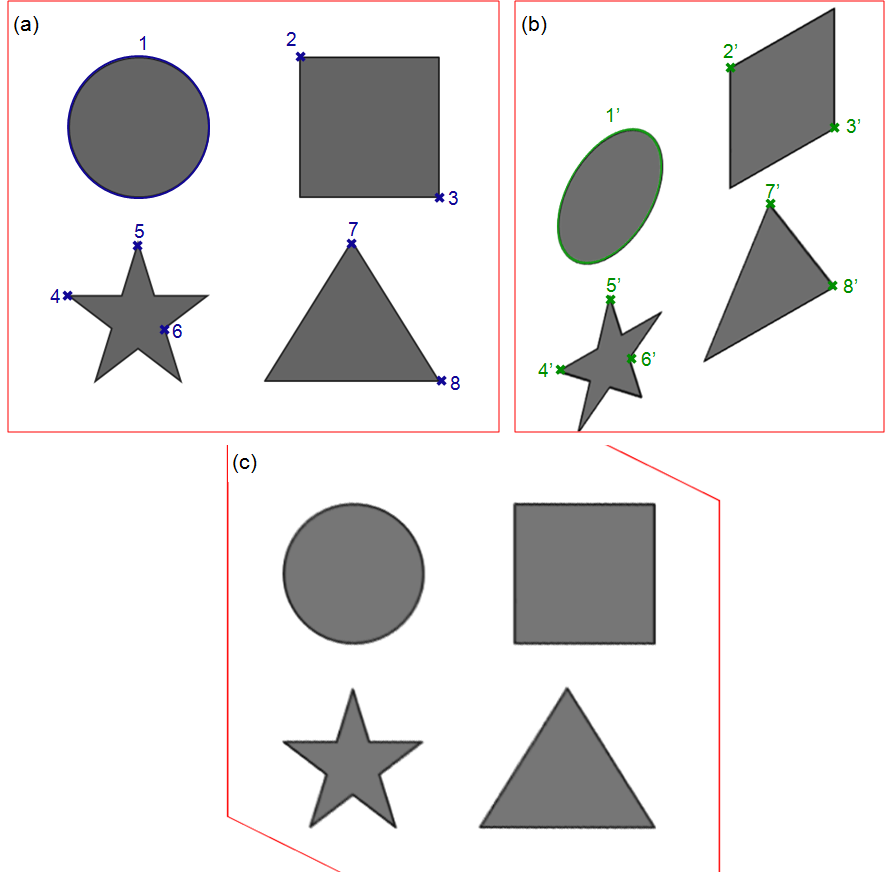
\includegraphics[height=296pt,width=300pt]{images/fig_img-reg}
    \caption{Possíveis pontos de controle: (a) Imagem de referência e
      (b) Imagem a ser registrada; (c) Imagem
      registrada.}\label{fig:img-reg}
  \end{center}
\end{figure}

Existe uma técnica de processamento de imagens que permite a detecção
e extração de pontos de controle invariáveis a ruído de imagem,
rotação, traslação, escala, e de forma parcial a mudanças de
iluminação e de perspectivas, chamada transformada SIFT (\textit{Scale
  Invariant Feature Transform}). A transformada SIFT tem demonstrado
ser muito eficiente ao gerar grande número de pontos de controle que
conseguem cobrir densamente uma imagem.\cite{85}

Vários softwares usam a transformada SIFT no registro de imagens,
entre eles o FIJI. O FIJI é um versátil software livre de
processamento digital de imagens, que pode ser descrito como uma
distribuição do ImageJ, desenvolvido pelo \textit{National Institutes
  of Health} dos Estados Unidos. A versatilidade do FIJI está dada
pela sua natureza, pois ele é um software composto por
\textit{plugins} organizados em uma estrutura de menu coerente. Como
software livre ele permite que experientes desenvolvedores em Java
possam criar novos \textit{plugins}. Ao mesmo tempo, ele oferece um
ambiente de programação mais simples através de uma interface de
\textit{script}.\cite{86}

Outros softwares de processamento digital de imagem também usam o
registro de imagem entre suas rotinas. É de particular interesse o
software comercial AxioVision. Uma das aplicações do registro de
imagens por este software é na fabricação de mosaicos. Esta técnica
tem como restrição um alinhamento imperfeito entre as direções
\textit{x} e \textit{y} da platina do microscópio e da imagem formada
pela câmera, fazendo com que os campos capturados fiquem
desalinhados.\cite{74} O AxioVision resolve este problema através de
uma função chamada \textit{Stitching}, a qual se baseia no registro de
imagens para alinhar os ladrilhos do mosaico. Além disso, este
software tem outra função chamada \textit{Geometric Correction} que
permite registrar imagens a uma imagem de referência.\cite{48}

\subsubsection{Delineação}

Outra operação comum de pré-processamento é a delineação. Imagens
obtidas por microscopia ótica apresentam valores de tonalidades
intermediários nas bordas dos objetos, devido a restrições de
resolução do sistema de formação da imagem. Assim, as fronteiras dos
objetos em lugar de serem uma linha de transição abrupta passam a ser
uma faixa de transição suave entre as tonalidades vizinhas.\cite{87}
Isto traz como consequência que, na hora de segmentar os objetos, seja
gerada uma fase espúria em forma de "halo" ao redor dos objetos. Este
fenômeno é conhecido como "efeito halo" e dificulta o correto
reconhecimento de regiões numa imagem.\cite{52}

Este problema é comumente reduzido utilizando uma técnica de
delineação. A delineação não é mais que um filtro inteligente que
varre a imagem procurando as transições entre fases e virtualmente
decidindo a qual fase os pixels pertencem. Para isto ele cria um
limiar ($m$) onde todos os pixels abaixo deste limiar pertencem a uma
fase e os acima dele pertencem à outra
(Figura~\ref{fig:transf-delin}). Já os pixels que se encontram fora
destas faixas de transição ficam praticamente inalterados.

\begin{figure} [h]
  \begin{center}
    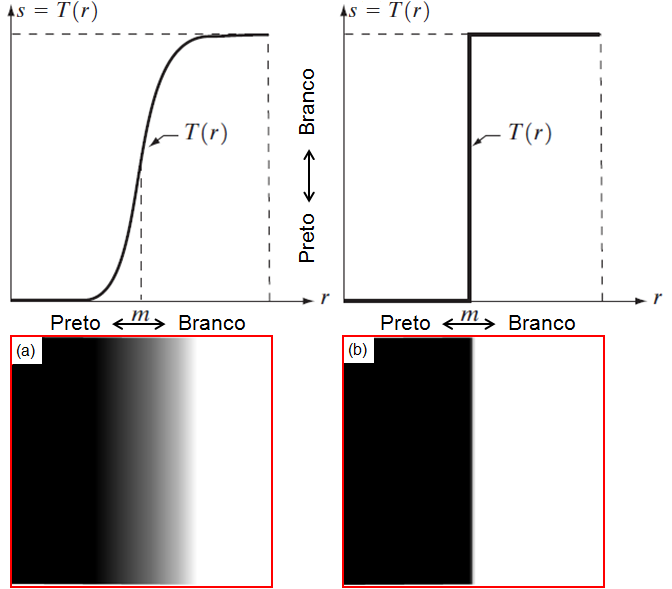
\includegraphics[height=307pt,width=350pt]{images/fig_transf-delin}
    \caption{Função de transformação para o realce do brilho nas
      bordas dos objetos.\cite{88}}\label{fig:transf-delin}
  \end{center}
\end{figure}

Um exemplo esquemático disto pode ser observado na
Figura~\ref{fig:transf-delin}, onde dois objetos vizinhos com
tonalidades diferentes (preto e branco) apresentam uma zona de
transição (Figura~\ref{fig:transf-delin}a). Após aplicar uma
delineação na imagem a transição passa a ser abrupta
(Figura~\ref{fig:transf-delin}b), como esperado, aumentando o
contraste entre os objetos.

Assim, esta técnica é empregada com bastante frequência quando a
separação de objetos na etapa de segmentação é crítica. Isto pode ser
observado claramente na Figura~\ref{fig:img-delin} onde uma imagem
multimodal de sínter de minério de ferro está prestes a ser
delineada. Da Figura~\ref{fig:img-delin}a é possível notar que o
contraste entre as fases com tonalidades mais cinzas (silicatos
vs. ferritos e ferritos vs. magnetita) não é tão bom como o contraste
entre a fase mais branca e o resto (silicatos, ferritos e magnetita)
vs. hematita. Após a delineação pode ser observado que os vales entre
os picos no histograma das fases mais cinzas diminuíram muito. Ao
mesmo tempo, na região ampliada da imagem, percebe-se um aumento do
contraste entre as fases.

\begin{figure} [h]
  \begin{center}
    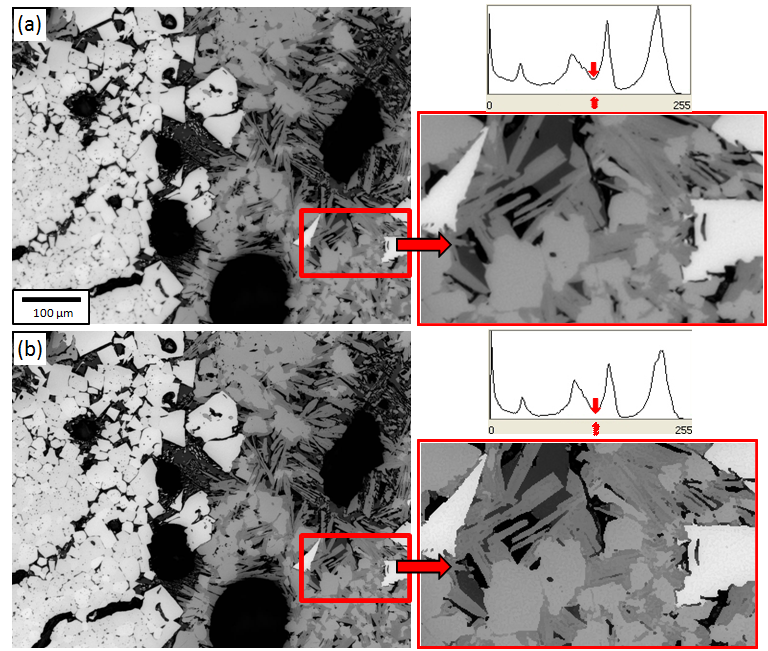
\includegraphics[height=297pt,width=350pt]{images/fig_img-delin}
    \caption{Delineação: (a) Imagem original, seu histograma e uma
      visão ampliada da região demarcada em vermelho; (b) Imagem
      delineada, seu histograma e a ampliação da mesma região
      demarcada em vermelho.\cite{74}}\label{fig:img-delin}
  \end{center}
\end{figure}

\subsubsection{Filtro Mediana}

Os ruídos aleatórios aparecem com muita frequência nas imagens. Estes
ruídos podem ser gerados por mal funcionamento dos dispositivos de
captura ou por falta de iluminação.\cite{89} Os pixels corrompidos ou
são alterados para o valor máximo da tonalidade, ou têm só alguns
\textit{bits} alterados, causando uma diferença brusca de tons entre
estes pixels e seus vizinhos. Quando os pixels são alternadamente
modificados para $0$ ou o máximo (255 em imagens de 8 bit), este ruído
é chamado de ruído sal-e-pimenta, devido a sua aparência.

Para este tipo de ruído o filtro mais eficiente é o filtro
mediana.\cite{90} A mediana, além de eliminar eficientemente o ruído
aleatório, preserva o contorno dos objetos da imagem.\cite{91}
Portanto, este filtro é de grande importância na etapa de
pré-processamento ao eliminar defeitos da adquisição e assim ajudando
na segmentação.

A mediana consiste num \textit{kernel} (Figura~\ref{fig:form-median})
de tamanho $n \times m$ que ordena os pixels em ordem crescente de
intensidade e escolhe como saída o valor mediano (aquele que esta no
centro da sequência). Como mostra a Figura~\ref{fig:form-median}, o
pixel central do \textit{kernel} (245) será substituído pelo valor que
está no centro da sequência ordenada (98). Neste exemplo observasse
que quando $n \times m$ é ímpar, a mediana é o próprio elemento
central da sequência ordenado. Nos casos em que $n \times m$ é par, a
mediana é calculada pela média aritmética dos dois elementos mais
próximos do centro.\cite{92}

\begin{figure} [h]
  \begin{center}
    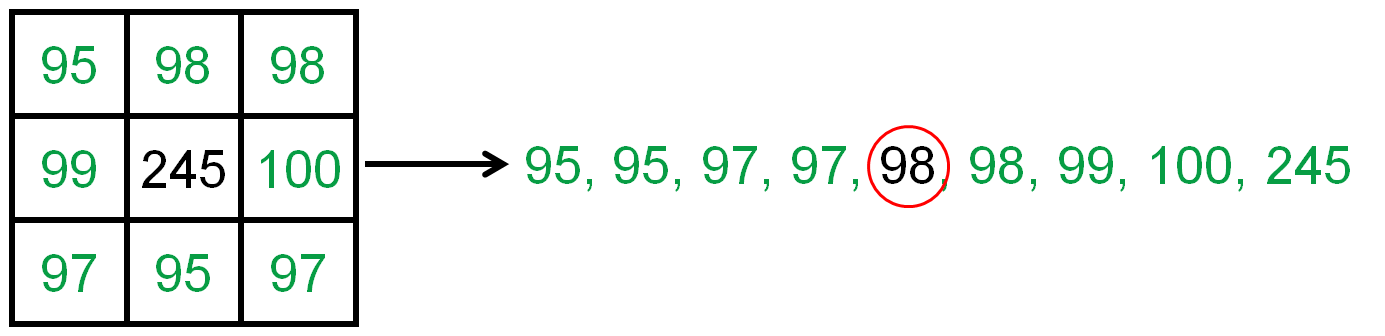
\includegraphics[height=73pt,width=300pt]{images/fig_form-median}
    \caption{Exemplo de um filtro mediana de tamanho
      3x3.}\label{fig:form-median}
  \end{center}
\end{figure}

O filtro mediana pode ser observado em ação na
Figura~\ref{fig:img-median}. Nesta figura temos uma imagem esquemática
com um ruído do tipo sal-e-pimenta
(Figura~\ref{fig:img-median}a). Sobre a mesma é aplicado um filtro
mediana de tamanho $3 \times 3$, onde os pixels com tonalidades muito
diferentes dos vizinhos foram eliminados
(Figura~\ref{fig:img-median}b). Contudo, ainda pode ser observado
pequenos defeitos residuais nas bordas dos objetos e da imagem, isto
se deve à característica do filtro de não alterar os contornos dos
objetos.

\begin{figure} [h]
  \begin{center}
    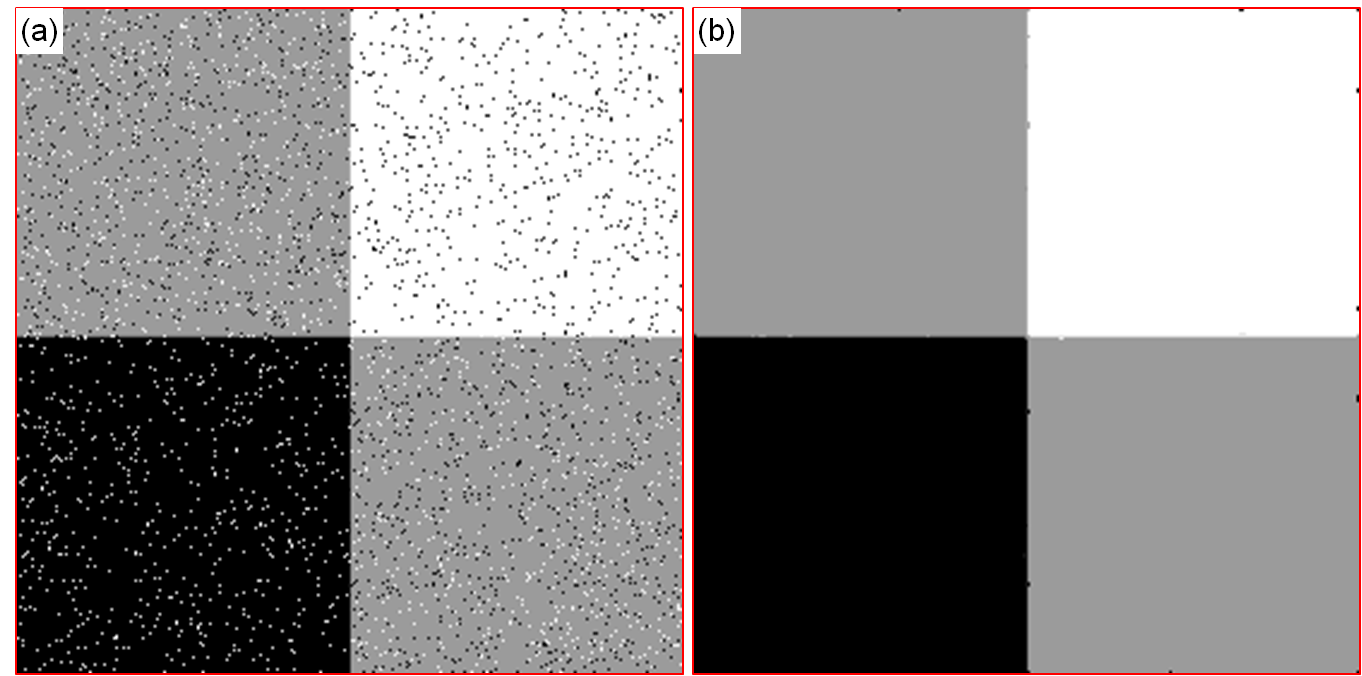
\includegraphics[scale=0.25]{images/fig_img-median}
    \caption{Uso do filtro mediana: (a) Imagem esquemática com ruído
      sal-e-pimenta; (b) Imagem esquemática com ruído reduzido pelo
      filtro mediana de tamanho 3x3.\cite{78}}\label{fig:img-median}
  \end{center}
\end{figure}

% ~\n~ ...
% \newpage

\subsection{Técnicas de segmentação}

Alguns psicólogos alemães no inicio do século XX, Khler, Wertheimer e
Kofftka, introduziram o princípio da segmentação. Eles mostraram que o
ser humano, no nível da visão, efetua agrupamentos sobre o que ele
percebe, baseados na proximidade, similaridade, e
continuidade.\cite{93} Entende-se por segmentação o processo de
divisão de uma imagem em suas partes ou objetos constituintes, sendo
uma das tarefas mais difíceis na análise de imagens.\cite{94}

A segmentação é uma tarefa básica no processo de análise de imagens,
mas não é fácil traduzir para o computador o sofisticado processo de
seleção e agrupamento realizado pela visão humana na identificação de
regiões semelhantes. Várias dificuldades estão presentes nesse
processo como a complexidade da textura, a irregularidade da
iluminação e as imprecisões das regiões das bordas. O problema de
segmentação torna-se particularmente difícil devido à textura da
imagem. Métodos de agrupamento baseados na cor podem alcançar
resultados satisfatórios quando as regiões que se deseja segmentar são
homogêneas. Porém, cenas naturais são complexas pela riqueza de
variações tonais e texturas presentes.\cite{95}

A segmentação de imagens tem sido um problema amplamente discutido no
campo de análise de imagens digitais. Existem diversas técnicas de
segmentação, dentre as quais se encontram:

 \begin{enumerate}[label=(\roman{*})]
   \item Segmentação por faixa tonal ou limiarização ;\cite{96,97,98}
   \item Segmentação por contornos;\cite{99,100}
   %\item Segmentação por morfologia matemática (\textit{watershed});\cite{103,104}
   \item Segmentação por crescimento de regiões;\cite{101,102}
   %\item Segmentação por textura;\cite{105}
   \item Entre outras, tais como \textit{watershed}, segmentação por
     textura, segmentação por entropia, etc.\cite{103,104,105,106,107}
\end{enumerate}

Categoricamente, não existe um método ideal e genérico de segmentação
que seja sempre o melhor.\cite{52} A segmentação costuma ser a etapa
crítica da sequência padrão de PADI. Uma segmentação adequada
praticamente garante o sucesso no reconhecimento e na identificação
dos objetos de interesse sobre os quais será feita a análise.\cite{88}

\subsubsection{Limiarização}

A técnica de segmentação mais simples e a mais utilizada é a
segmentação por faixa tonal, também chamada limiarização ou
\textit{thresholding}. A limiarização usa o tom dos pixels para
separar objetos (regiões de pixels contíguos com tons dentro de uma
faixa tonal delimitada) de outros usando um limiar ou tom de
corte.\cite{72} Este método é implementado de forma interativa na
maior parte das vezes, porém alguns autores tem se esforçado por criar
inovadores métodos de limiarização automática.\cite{98,108}

No caso de diferençar objetos de um fundo, utiliza-se a limiarização
bimodal, a qual discrimina duas fases na imagem, o fundo e os
objetos. Esta segmentação parte da hipótese de que a imagem apresenta
um histograma bimodal e, portanto, que os objetos podem ser separados
do fundo por uma simples operação que compara o tom dos pixels da
imagem com um valor de limiar (L). Supondo que a imagem $f(x,y)$
corresponda a um histograma bimodal, então a imagem segmentada
$g(x,y)$ seria definida como:

\begin{align}
&g(x,y) =  \left\lbrace
	\begin{array}{c c} 
		1  
		& \text{se }(x,y) \; \textgreater \; \text{L} \\  
		0  
		& \text{se }(x,y) \; \le \; \text{L}
	\end{array}\right.
\end{align}

O resultado da limiarização seria uma imagem binaria, onde os pixels
com valor 1 correspondem aos objetos, enquanto os pixels com valor 0
correspondem ao fundo.

A Figura~\ref{fig:lim-bimod} mostra um exemplo simples de segmentação
por faixa tonal. Uma imagem de minério de ferro
(Figura~\ref{fig:lim-bimod}a), em 256 tons por canal RGB, obtida por
microscopia ótica, é segmentada por limiarização bimodal. Gera-se uma
imagem binária (Figura~\ref{fig:lim-bimod}b), através do tom de corte
(L=132) indicado em seu histograma (Figura~\ref{fig:lim-bimod}c), e a
fase mais clara (hematita) é separada do resto da imagem. Neste caso
específico, por razões metodológicas, o histograma mostrado pertence
apenas a um canal da imagem RGB.

\begin{figure} [h]
  \begin{center}
    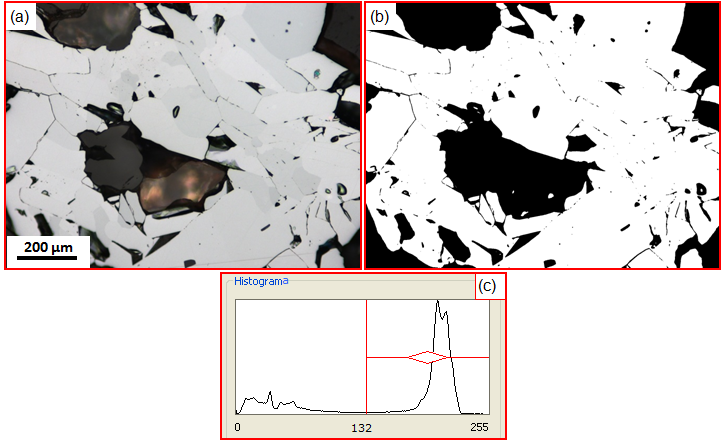
\includegraphics[height=245pt,width=400pt]{images/fig_lim-bimod}
    \caption{Exemplo de limiarização bimodal: (a) Imagem original; (b)
      Imagem binária; (c) Tom de corte no
      histograma.}\label{fig:lim-bimod}
  \end{center}
\end{figure}

A técnica de limiarização também é aplicável se for necessário
discriminar mais de uma faixa tonal na imagem, pois ela não está
restrita apenas a duas fases. Este tipo de limiarização é conhecido
como limiarização multimodal e gera tantas imagens binárias quantas
fases sejam segmentadas. Neste caso os pixels brancos da imagem
binária formam a fase de interesse, que fica entre os dois tons de
corte, e o fundo preto é o resto. Assim, supondo que a imagem $f(x,y)$
corresponda a um histograma multimodal então, neste caso, a imagem
segmentada $g(x,y)$ seria definida como:

\begin{align}
&~~~~~~~~~~~~~~~~~~~~~~~~~g_{i}(x,y) =  \left\lbrace
	\begin{array}{c c} 
		1  
		& \text{se } \text{L}_{i} \; \textless \; (x,y) \; \le \; \text{L}_{i+1} \\  
		0  
		& \text{se }\text{L}_{i} \; \ge \; (x,y) \; \textgreater \; \text{L}_{i+1}
	\end{array}\right. \\
&\text{onde ~$g_{i}(x,y)$ ~seria ~a $i-esima$ ~imagem ~binaria ~pertencente ~à ~$i-esima$} \nonumber\\
&\text{fase e;} \nonumber\\
&~~~~~~~~~~~~~~~~~~~~~~~~~g(x,y) = \bigcup\limits_{i=1}^n g_{i}(x,y) \\
&\text{o resultado ~final ~da limiarização ~multimodal, onde ~os pixels ~com ~valor ~$1$} \nonumber\\
&\text{correspondem ~às fases ~de interesse, enquanto ~os pixels ~com ~valor $0$ corres-} \nonumber\\
&\text{pondem ao resto.} \nonumber
\end{align}

A Figura~\ref{fig:2-6} mostra um exemplo de limiarização multimodal
para distinguir cinco fases. Uma imagem de sínter de minério de ferro
(Figura~\ref{fig:2-6}a) segmentada por limiarização pentamodal,
gerando uma imagem com 5 faixas (Figura~\ref{fig:2-6}b) através dos
quatros tons de corte (L=32, L=74, L=134, L=170) mostrados em seu
histograma (Figura~\ref{fig:2-6}c). A cada faixa foi atribuída uma
cor, para facilitar a visualização, correspondente à cor do histograma
entre seus respectivos tons de cortes.
 
 
\begin{figure} [h]
  \begin{center}
    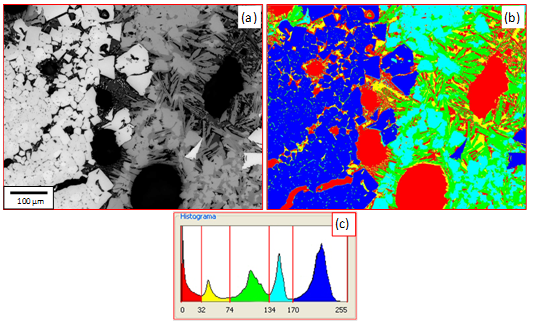
\includegraphics[height=243pt,width=400pt]{images/fig2-6}
    \caption{Exemplo de limiarização pentamodal: (a) Imagem original
      em 256 tons de cinza; (b) Imagem quinária com as fases
      diferençadas com cores; (c) Tons de corte no
      histograma.\cite{74}}\label{fig:2-6}
  \end{center}
\end{figure}

\vspace{20 mm}

\subsubsection{Segmentação por Contornos}

Um contorno é uma mudança brusca da tonalidade entre duas regiões
relativamente homogêneas. Ele pode aparecer como uma sequência de
pontos, uma linha, um segmento, uma curva ou uma forte variação do
nível de cinza médio.\cite{88}

Uma das técnicas de detecção de bordas mais usadas consiste no
processamento de uma imagem a partir de um operador de derivada
local. Exemplos destes operadores são o gradiente e o laplaciano,
operadores de derivada de primeira e segunda ordem, frequentemente
utilizados nas técnicas de detecção de bordas.\cite{88}

A segmentação por contornos simula o funcionamento da visão
humana. Ela detecta as bordas dos objetos, a partir das quais constrói
seus contornos, considerando como objeto a região dentro do
contorno.\cite{72}

Entre as técnicas de segmentação por contornos, uma das mais
conhecidas é a proposta por Canny.\cite{100} Este autor desenvolveu um
processo de detecção de bordas a partir de critérios de quantificação
de desempenho de operadores de bordas conhecidos como os critérios de
detecção e de localização. Estes critérios de desempenho ainda estão
sujeitos ao critério de resposta múltipla, que corresponde ao fato de
que deve existir, na saída do operador, uma única resposta para uma
única borda. Para que os critérios sejam aproximadamente atendidos,
Canny aproxima o operador ótimo, obtido a partir dos três critérios de
desempenho, pela primeira derivada da função Gaussiana. Em complemento
a este operador foram propostos dois processos conhecidos como:

\begin{enumerate}[label=(\roman{*})]
  \item Supressão não máxima (supressão de valores de pixels que não
    forem máximos locais na direção transversal à borda), que causaria
    um afinamento da borda, atendendo à injunção de resposta múltipla; e
  \item Uma limiarização adaptativa (histerese) com ``complementação
    de bordas", para eliminar a fragmentação dos contornos das
    bordas.\cite{109}
\end{enumerate}

A Figura~\ref{fig:seg-canny} mostra um exemplo de detecção de
borda. Uma imagem em luz polarizada de minério de ferro
(Figura~\ref{fig:seg-canny}a) obtida por microscopia ótica, é
segmentada pelo método de Canny. Gera-se uma imagem binária
(Figura~\ref{fig:seg-canny}b) com as bordas dos cristais de
hematita. Contudo, este método é sensível aos riscos, às bordas
espúrias provenientes de ruído e à textura da imagem, conforme
indicado pelas setas verdes nas imagens da
Figura~\ref{fig:seg-canny}. Por outro lado, o método do Canny gera
muitas bordas descontínuas.

\begin{figure} [h]
  \begin{center}
    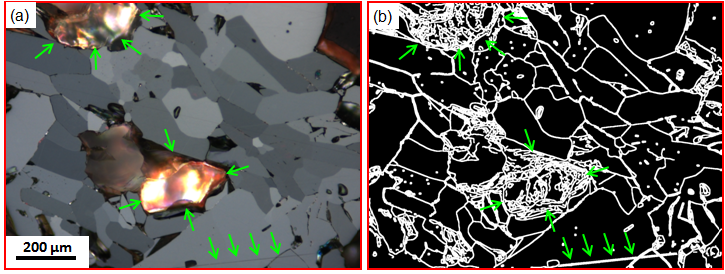
\includegraphics[height=148pt,width=400pt]{images/fig_seg-canny}
    \caption{Exemplo de detecção de bordas pelo método de Canny: (a)
      Imagem original; (b) Imagem binária com as bordas dos cristais
      de hematita.}\label{fig:seg-canny}
  \end{center}
\end{figure}

\subsubsection{Crescimento de Regiões}

Algoritmos de segmentação por crescimento de regiões agrupam pixels ou
sub-regiões em regiões maiores, partindo de um conjunto de pontos
iniciais (sementes) que crescem anexando pixels ou regiões adjacentes
que possuam propriedades similares, como, por exemplo, tom de cinza,
textura ou cor.\cite{110} Porém, o que define o tipo de crescimento de
regiões é o critério de parada do algoritmo. No presente trabalho
serão usados dois tipos de crescimento de regiões:

\begin{enumerate}[label=(\roman{*})]
  \item Crescimento de regiões usando a distância espectral como
    parâmetro de cor e;
  \item Crescimento de regiões usando a heterogeneidade como parâmetro
    de textura.
\end{enumerate}

Inicialmente, vai ser explicado o método tradicional de crescimento de
regiões. A formulação básica adotada para este tipo de abordagem é
dada considerando \textit{I} como uma imagem onde a segmentação é a
decomposição de \textit{I} em \textit{n} regiões \textit{R}$_{1}$,
\textit{R}$_{2}$, ..., \textit{R}$_{n}$ de tal forma que:

\begin{align}
 &I = \bigcup\limits_{i=1}^n R_{i}\\
 &R_{i} ~ \text{é uma região conexa, $1, 2, ..., n$}\\
 &R_{i} \bigcap R_{j} = \emptyset ~ \forall i \neq j\\
 &P\left(R_{i}\right)= \text{verdadeiro ~} \forall i\\
 &P\left(R_{i} \bigcap R_{j}\right)=\text{falso~} \forall i \neq j
\end{align}

Pode existir um número de possíveis partições, mas a seleção de um
conjunto adequado de regiões depende da escolha da propriedade
\textit{P} associada à região, ou seja, do predicado de uniformidade
dos pixels da região.\cite{88}

A técnica consiste nas seguintes etapas:

\begin{enumerate}[label=(\roman{*})]
  \item Escolha dos pixels-sementes (pontos ou simplesmente sementes);
  \item Escolha do limiar que separará as regiões; e
  \item Crescimento das regiões.
\end{enumerate}

A escolha dos pixels-sementes geralmente é feita baseando-se na
natureza do problema. A escolha destes pontos é importante, pois as
regiões crescerão ao redor deles.

Para entender bem o método, vai ser utilizado um exemplo. Neste
exemplo trabalha-se com dois cenários: o primeiro com duas sementes,
cada uma, com o valor mínimo e máximo do tom de cinza da imagem. Já no
segundo cenário será usada uma terceira semente com o valor médio dos
tons de cinza da imagem.

Como anteriormente definido, o crescimento das regiões em si consiste
em se fazer o agrupamento de pixels por similaridade baseado em alguns
critérios como intensidade dos tons de cinza, textura, cor, etc. Aqui,
é utilizada a intensidade dos tons de cinza como exemplo. Então
pode-se dizer que:

\begin{align}
  &\text{Se}\mid P\left(x,y\right)-P\left(x_{1},y_{1}\right)\mid \textless t\text{, então $P\left(x,y\right)\in R_{1}$ senão,}\\
  &\text{Se}\mid P\left(x,y\right)-P\left(x_{2},y_{2}\right)\mid \textless t\text{, então $P\left(x,y\right)\in R_{2}$ senão,}\\
  &... \nonumber\\
  &\text{Se}\mid P\left(x,y\right)-P\left(x_{n},y_{n}\right)\mid
  \textless t\text{, então $P\left(x,y\right)\in
    R_{n}$;}
\end{align}

onde $P(x,y)$ é a intensidade de cinza em um ponto $(x,y)$ da tabela
de intensidades; $n$ são as sementes; $R_{i}$, com $1 \leqslant i
\leqslant n$, são as regiões e; $t$ é o valor do limiar.

Um exemplo simples do funcionamento do crescimento de regiões clássico
pode ser observado na Figura~\ref{fig:ex-cresregio}. Na
Figura~\ref{fig:ex-cresregio}a pode-se observar uma imagem em tom de
cinza onde são tomados como sementes os pontos $P(1,1) = 0$ e $P(2,3)
= 7$. Como se pode observar, estas sementes representam os extremos da
faixa tonal da imagem, isso combinado com um limiar $t = 3$ faz com
que alguns pixels não sejam incluídos em nenhuma das duas regiões
possíveis $(R_{1}$ e $R_{2})$
(Figura~\ref{fig:ex-cresregio}b). Contudo, se for tomada uma terceira
semente $P(4,4) = 3$ e for mantido com o mesmo limiar $t = 3$, seria
criada uma terceira região $(R_{3})$ incluindo os pixels antes
rejeitados (Figura~\ref{fig:ex-cresregio}c). É interessante também
notar que, se for escolhido um valor de limiar mais alto, por exemplo
$t = 8$, só haveria uma região no exemplo em questão. Esse exemplo
serve para mostrar a importância de uma escolha adequada dos limiares,
bem como dos pixels-sementes para ter o sucesso esperado no método de
crescimento de regiões.

\begin{figure} [h]
  \begin{center}
    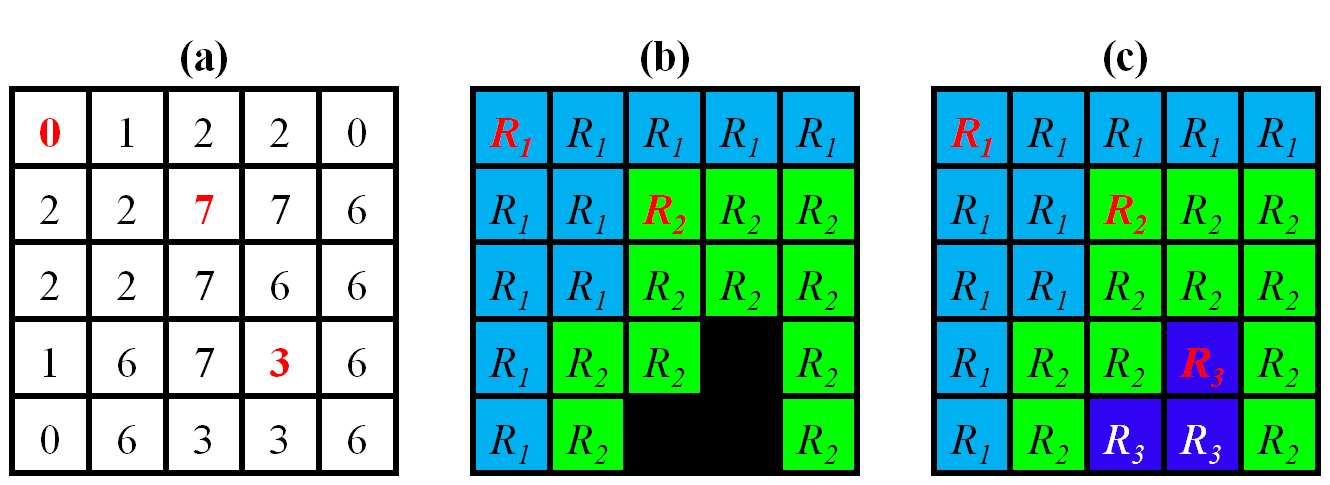
\includegraphics[height=146pt,width=400pt]{images/fig_ex-cresregio}
    \caption{Exemplo de crescimento de regiões com $t =3$: (a) Imagem
      em tons de cinza; (b) Duas regiões $(R_{1}$ e $R_{2})$ separadas
      com $n = 2$ sementes (em vermelho); (c) Três regiões $(R_{1}$,
      $R_{2}$ e $R_{3})$ separadas com $n = 3$ sementes (em
      vermelho).}\label{fig:ex-cresregio}
  \end{center}
\end{figure}

\subsection{Pós-processamento}

Frequentemente o resultado da segmentação não é tão bom quanto
esperado, sendo necessário aplicar rotinas de pós-processamento para
corrigir os defeitos recorrentes da segmentação. Estas rotinas
generalmente se baseiam na implementação de operações lógicas e
morfológicas.

\subsubsection{Operações Lógicas}

Na segmentação a imagem é binarizada, ou seja, cada pixel que compõe a
imagem ou bem é branco (com valor $1$ ou $255$ dependendo do
software), ou bem é preto (com valor $0$). Assim, resulta fácil
imaginar que operações lógicas (também conhecidas como operações
booleanas em homenagem a seu criador Boole) possam ser aplicadas entre
os pixels das imagens.

As operações lógicas são operações pontuais entre imagens binárias,
realizadas por operadores lógicos ($\otimes$) que varrem as imagens de
entrada, operando pixel a pixel, gerando uma imagem de saída
(Figura~\ref{fig:logic-puntual}) onde cada pixel é preservado ou
invertido.\cite{72} Ou seja:

\begin{align}
 &\textit{\textbf{A}} \otimes \textit{\textbf{B}} = \textit{\textbf{C}}
\end{align}

onde \textit{\textbf{A}}, \textit{\textbf{B}} e \textit{\textbf{C}}
são imagens e $\otimes$ é um operador lógico (AND, OR, XOR).

\begin{figure} [h]
  \begin{center}
    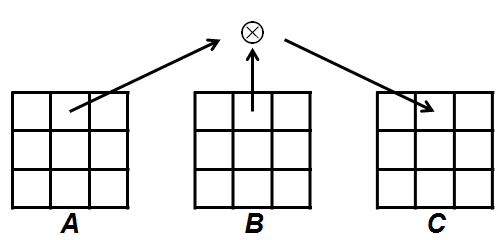
\includegraphics[height=119pt,width=250pt]{images/fig_logic-puntual}
    \caption{Operações lógicas pixel a
      pixel.}\label{fig:logic-puntual}
  \end{center}
\end{figure}

As três operações lógicas básicas são o complemento (NOT), a união
(OR) e a intersecção (AND), a partir das quais qualquer outra operação
lógica pode ser definida. Na Figura~\ref{fig:logic-basic} pode ser
observado como a operação NOT inverte todos os pixels da imagem de
entrada, gerando uma imagem de saída que é seu negativo. Ao mesmo
tempo, a operação OR realiza a união das duas imagens de entrada,
produzindo uma imagem de saída onde são brancos somente os pixels que
são brancos em pelo menos uma das imagens de entrada. Finalmente, a
operação AND faz a intersecção entre as duas imagens de entrada,
produzindo uma imagem de saída onde são brancos somente os pixels que
são brancos em ambas as imagens de entrada.

\begin{figure} [h]
  \begin{center}
    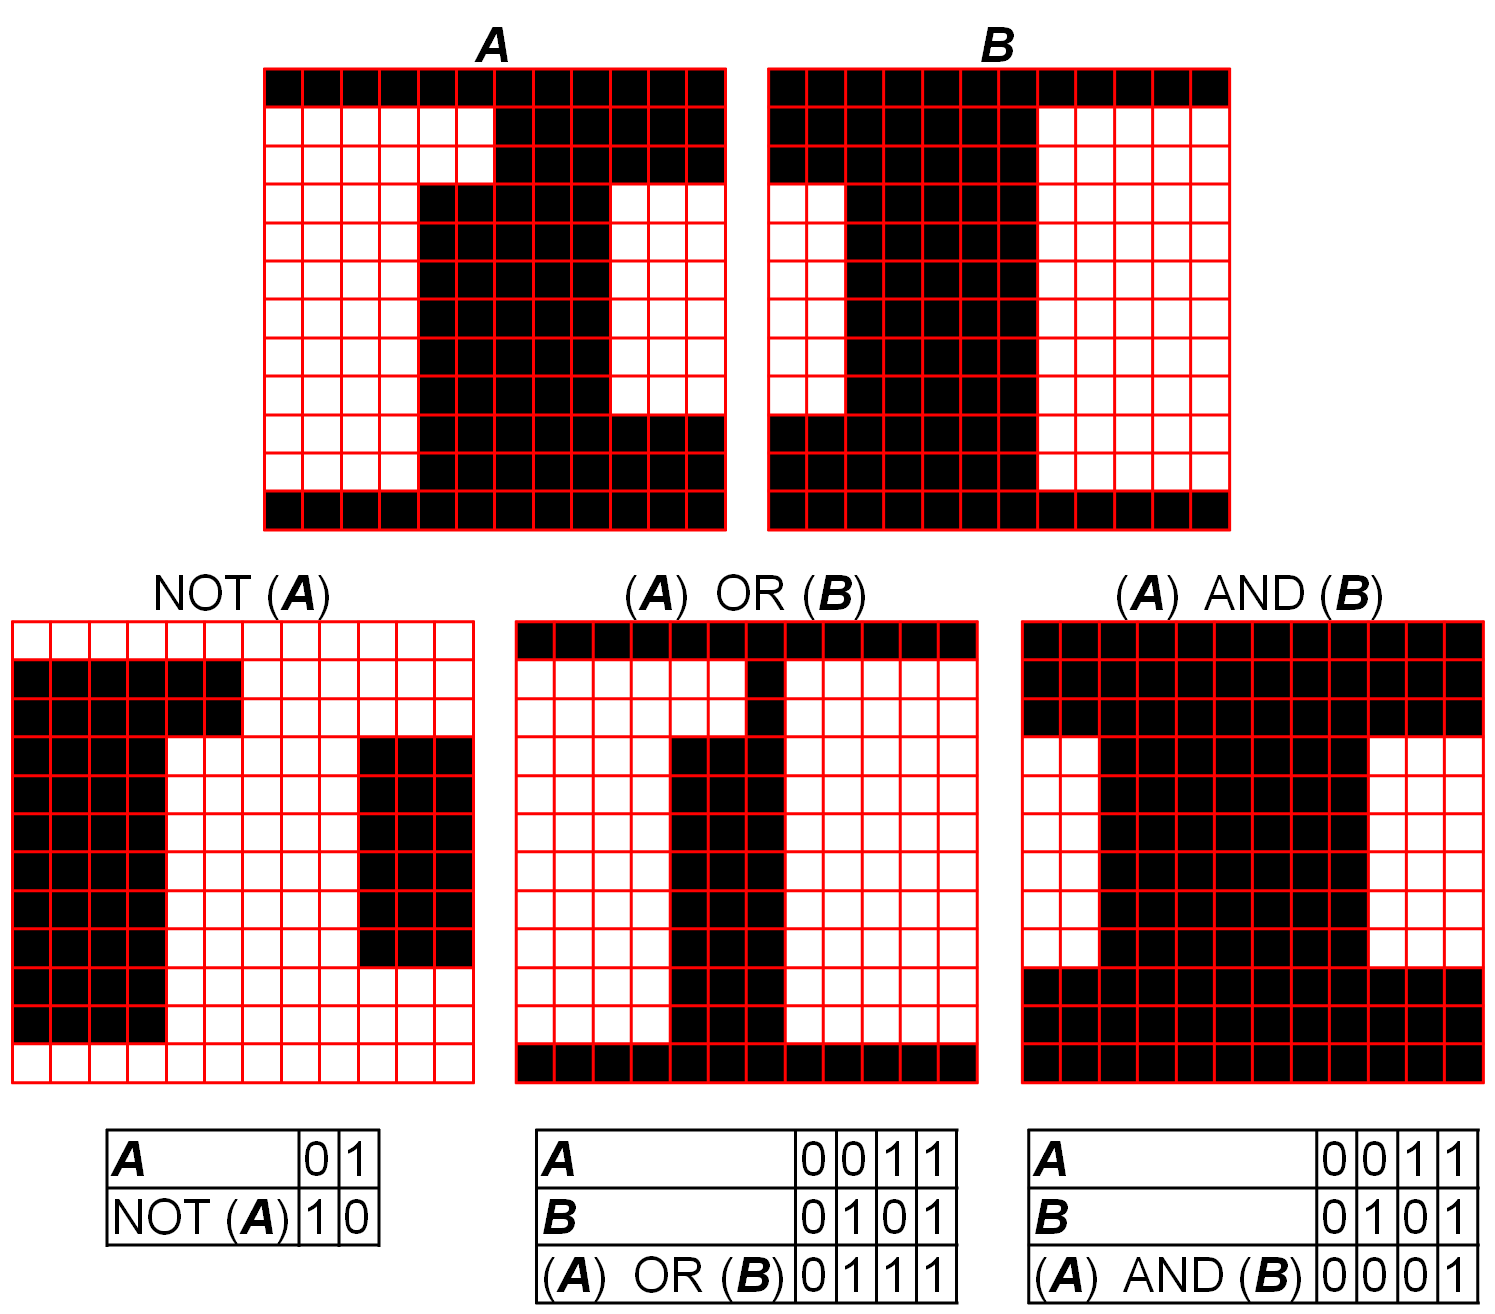
\includegraphics[height=308pt,width=350pt]{images/fig_logic-basic}
    \caption{Operações lógicas básicas (NOT, OR e
      AND).}\label{fig:logic-basic}
  \end{center}
\end{figure}

Outra operação lógica, derivada dessas operações básicas, também
bastante utilizada, é o OR exclusivo (XOR). Esta operação não é mais
que a intersecção entre a saída de um OR e o complemento da saída de
um AND. Ou seja:

\begin{align}
 &(\textit{\textbf{A}}) \;  XOR \; (\textit{\textbf{B}}) = \left\lbrace (\textit{\textbf{A}}) \; OR \; (\textit{\textbf{B}}) \right\rbrace \; AND \; \left\lbrace  NOT \; \left[ (\textit{\textbf{A}}) \; AND \; (\textit{\textbf{B}}) \right] \right\rbrace
\end{align}

Na Figura~\ref{fig:logic-xor} pode ser observado como a operação XOR
gera uma imagem de saída onde unicamente são brancos aqueles pixels
que eram brancos em somente uma das imagens de entrada. Na prática, o
operador XOR calcula a diferença entre as duas imagens binárias (não
confundir com a operação de subtração).
 
\begin{figure} [h]
  \begin{center}
    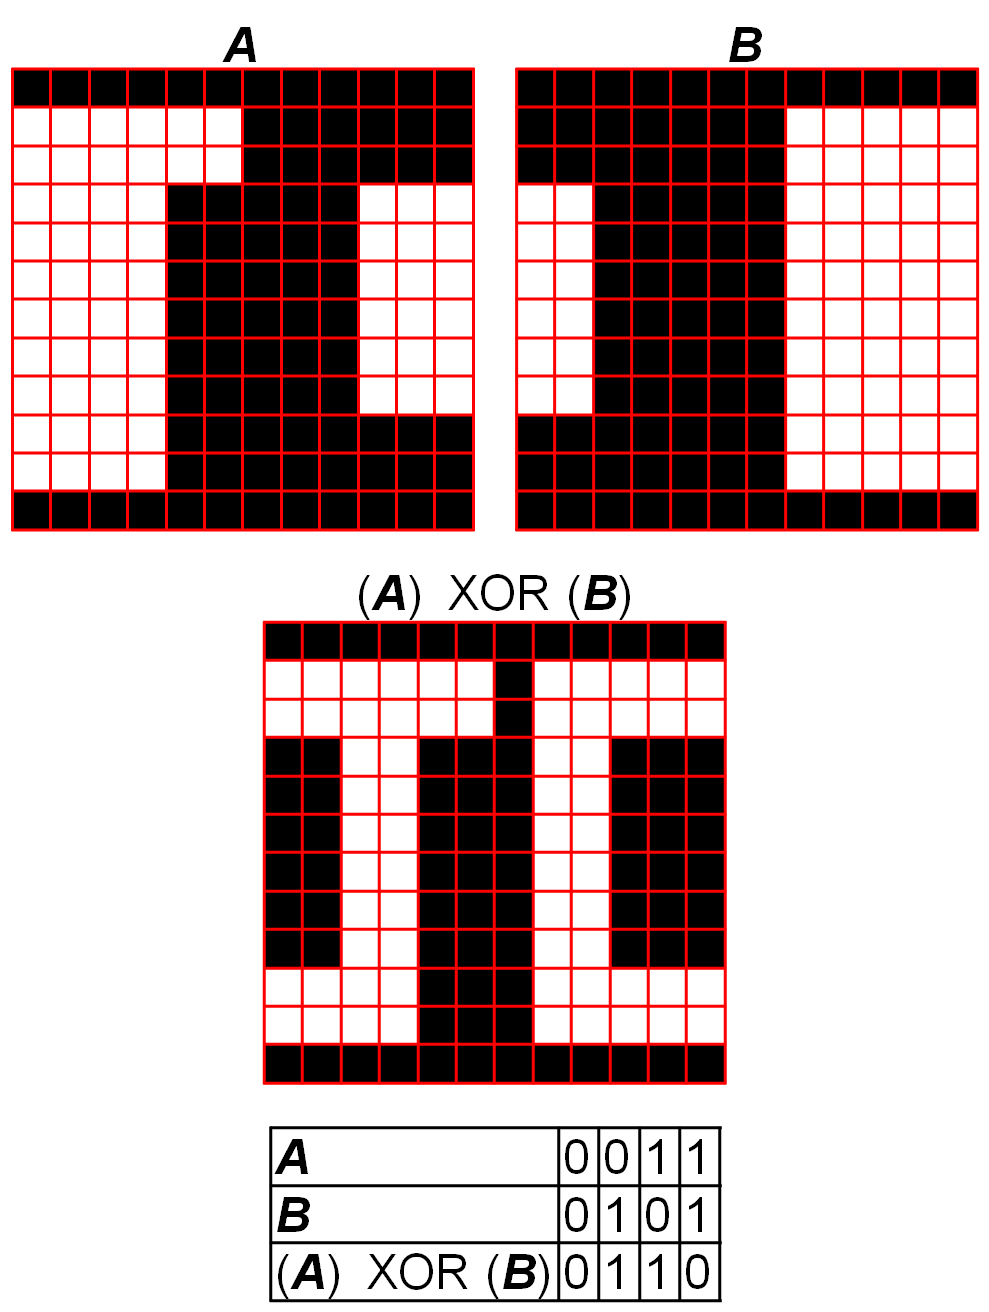
\includegraphics[height=309pt,width=233pt]{images/fig_logic-xor}
    \caption{Operação lógica XOR.}\label{fig:logic-xor}
  \end{center}
\end{figure}

Como pode ser observado, os operadores AND, OR e XOR requerem duas
imagens de entrada e geram uma imagem de saída. Porém, no caso
particular do operador NOT somente requer uma imagem de entrada para
gerar uma imagem de saída. Assim, podem-se criar infinitas combinações
lógicas com estes operadores a fim de corrigir defeitos da segmentação
em imagens binárias. Contudo, é bom ter presente a importância da
ordem dos operadores, deste modo é de vital importância o uso de
parêntesis para esclarecer a ordem e prioridade das operações.

Até aqui vimos o uso dos operadores lógicos em imagens binárias, porém
eles também podem ser usados em imagens em tom de cinza. O uso de uma
imagem binária como máscara para modificar uma imagem em tom de cinza
é uma prática comum no processamento de imagens.

\subsubsection{Operações Morfológicas}

A morfologia matemática concentra seus esforços no estudo das
estruturas geométricas das entidades presentes numa imagem.\cite{111}
As operações morfológicas podem ser aplicadas em várias áreas de
processamento e análise de imagens, com objetivos tão distintos como
realce, filtragem, segmentação, detecção de bordas, esqueletização,
afinamento, dentre outras.\cite{91}

Assim como as operações lógicas, as operações morfológicas também têm
suas operações básicas (traslação, reflexão, complemento, erosão e
dilatação). Estas operações consistem em extrair as informações
relativas à geometria dos objetos de uma imagem, apoiando-se numa
pequena imagem binária, denominada elemento estruturante. O elemento
estruturante varre a imagem de entrada, preservando ou invertendo o
valor do pixel central da vizinhança, na imagem de saída, em função de
seus vizinhos.\cite{72} Portanto, a base das operações morfológicas é
a teoria de conjuntos. Neste caso particular em que tanto as imagens
de entrada como o elemento estruturante são imagens binárias, os
conjuntos em questão pertencem ao espaço inteiro bidimensional
($\mathbb{Z}^{2}$).

Primeiramente procederemos a fazer as definições das operações
morfológicas básicas entre os conjuntos \textit{\textbf{A}} e
\textit{\textbf{B}}, pertencentes ao espaço $\mathbb{Z}^{2}$, onde $a$
e $b$ são suas respectivas componentes. O conjunto \textit{\textbf{A}}
é normalmente atribuído à imagem de entrada, quanto o conjunto
\textit{\textbf{B}} é normalmente atribuído ao elemento estruturante.

A primeira definição é a \underline{traslação} de \textit{\textbf{A}}
($\textit{\textbf{A}}_{x}$) em $x$ gerando a imagem
\textit{\textbf{C}}.\cite{88} Ou seja:

\begin{align}
 &\textit{\textbf{A}}_{x} = \left\lbrace \text{$c$; $c = a + x$ \: $\forall a \in A$} \right\rbrace
\end{align}

A \underline{reflexão} de \textit{\textbf{B}}
($\hat{\textit{\textbf{B}}}$), por sua vez, seria:

\begin{align}
 &\hat{\textit{\textbf{B}}} = \left\lbrace \text{$c$; $c = -b$ \: $\forall b \in B$} \right\rbrace
\end{align}

O \underline{complemento} de \textit{\textbf{A}}
($\textit{\textbf{A}}^{c}$):

\begin{align}
 &\textit{\textbf{A}}^{c} = \left\lbrace \text{$c$; \: $c \notin A$} \right\rbrace
\end{align}

A \underline{erosão} de \textit{\textbf{A}} por \textit{\textbf{B}}
(\textit{\textbf{A}} $\ominus$ \textit{\textbf{B}}):

\begin{align}
  &\textit{\textbf{A}} \ominus \textit{\textbf{B}} = \left\lbrace
    \text{$c$; \: $\textit{\textbf{B}}_{x} \subseteq A$}
  \right\rbrace\label{eq-erode}
\end{align}

o que, em outras palavras, significa que a erosão de
\textit{\textbf{A}} por \textit{\textbf{B}} resulta no conjunto dos
pontos $c$, da imagem de saída, tais que \textit{\textbf{B}},
trasladado ($\textit{\textbf{B}}_{x}$), está contido em
\textit{\textbf{A}}.

Finalmente a \underline{dilatação} de \textit{\textbf{A}} por
\textit{\textbf{B}} (\textit{\textbf{A}} $\oplus$
\textit{\textbf{B}}):

\begin{align}
 &\textit{\textbf{A}} \oplus \textit{\textbf{B}} = \left\lbrace \text{$c$; \: $\left[ (\hat{\textit{\textbf{B}}})_{x} \cap \textbf{\textit{A}} \right] \subseteq A$} \right\rbrace
\end{align}

ou seja, o processo de dilatação consiste em obter primeiramente a
reflexão de \textit{\textbf{B}} sobre sua origem e depois sua
traslação ($(\hat{\textit{\textbf{B}}})_{x}$). Deste modo, a dilatação
de \textit{\textbf{A}} por \textit{\textbf{B}} é o conjunto dos pontos
$c$, da imagem de saída, para os quais a intersecção de
$(\hat{\textit{\textbf{B}}})_{x}$ e \textit{\textbf{A}} está contido
em \textit{\textbf{A}}.

A erosão e a dilatação podem ser observadas mais facilmente na
Figura~\ref{fig:eroc-dilat}, onde uma imagem esquemática
(\textit{\textbf{A}}), de 12x12 pixel, é erodida (\textit{\textbf{C}})
e dilatada (\textit{\textbf{D}}) pelo elemento estruturante
(\textit{\textbf{B}}), de 3x3 pixel.

\begin{figure} [h]
  \begin{center}
    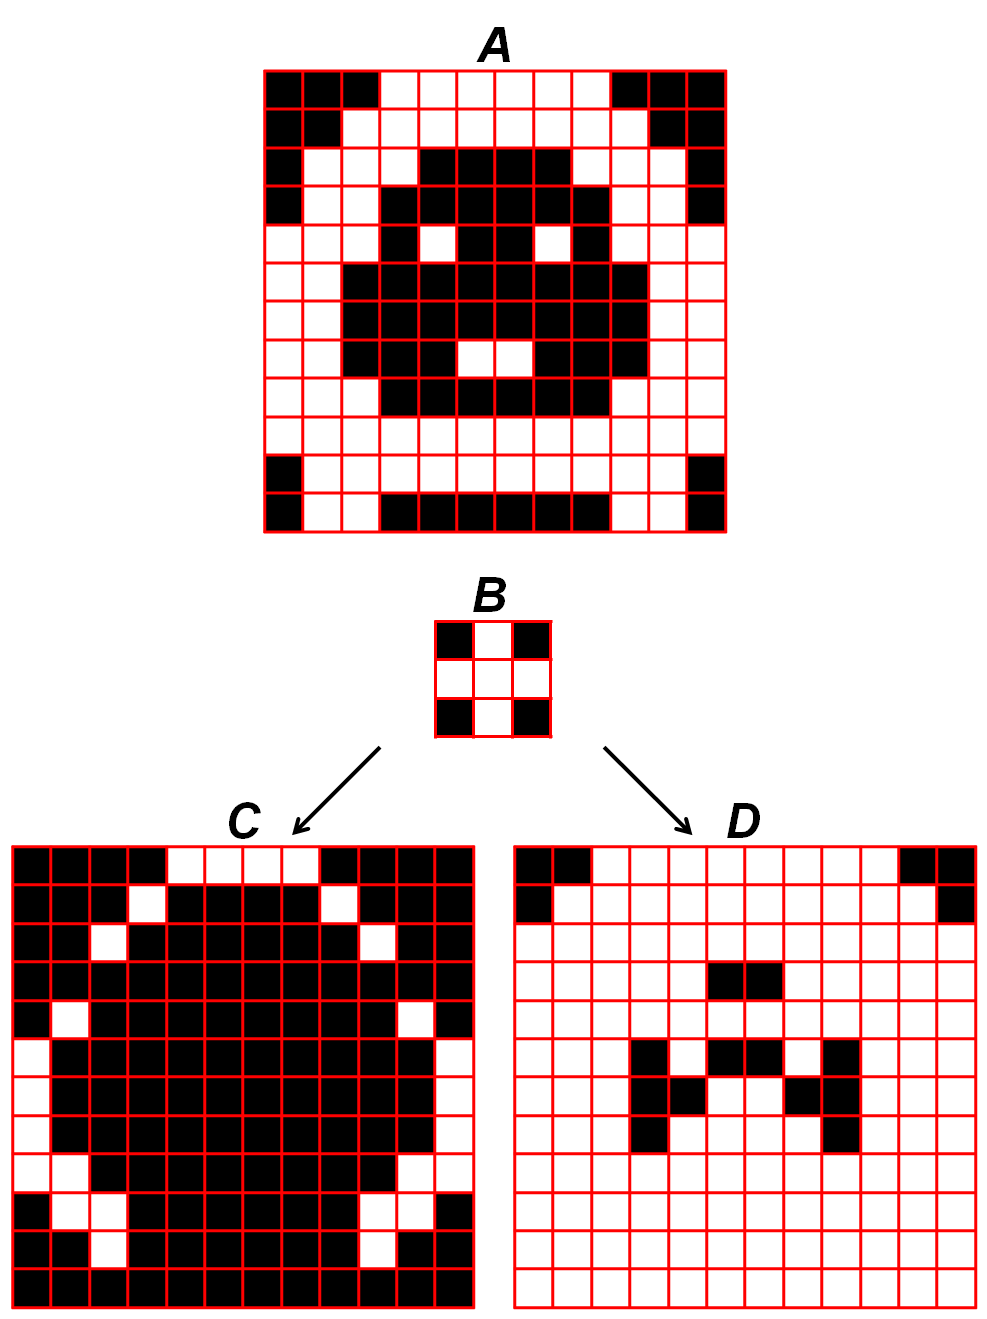
\includegraphics[height=334pt,width=250pt]{images/fig_eroc-dilat}
    \caption{Erosão e Dilatação.}\label{fig:eroc-dilat}
  \end{center}
\end{figure}

É bom ressaltar que alguns softwares de processamento digital de
imagens permitem ao usuário criar seus próprios elementos
estruturantes.\cite{112} Estes elementos estruturantes podem ter as
mais variadas formas e tamanhos, sendo a escolha do mais adequado
determinada somente em função do problema. No caso particular deste
exemplo (Figura~\ref{fig:eroc-dilat}) o elemento estruturante usado
(\textit{\textbf{B}}) é chamado de elemento de conectividade 4. Isto
se deve ao fato de que ele define uma vizinhança 3x3, sendo
considerados vizinhos do pixel central somente os 4 pixels adjacentes
a ele na horizontal e na vertical. Um outro elemento estruturante,
também muito utilizado e que também define uma vizinhança 3x3, é o
elemento de conectividade 8. Neste caso todos os 8 pixels adjacentes
ao pixel central são considerados seus vizinhos.

Combinando estas operações morfológicas básicas podem-se criar outras
novas e importantes operações morfológicas. Duas das mais importantes
são a abertura e o fechamento (Figura~\ref{fig:open-close}).

\begin{figure} [h]
  \begin{center}
    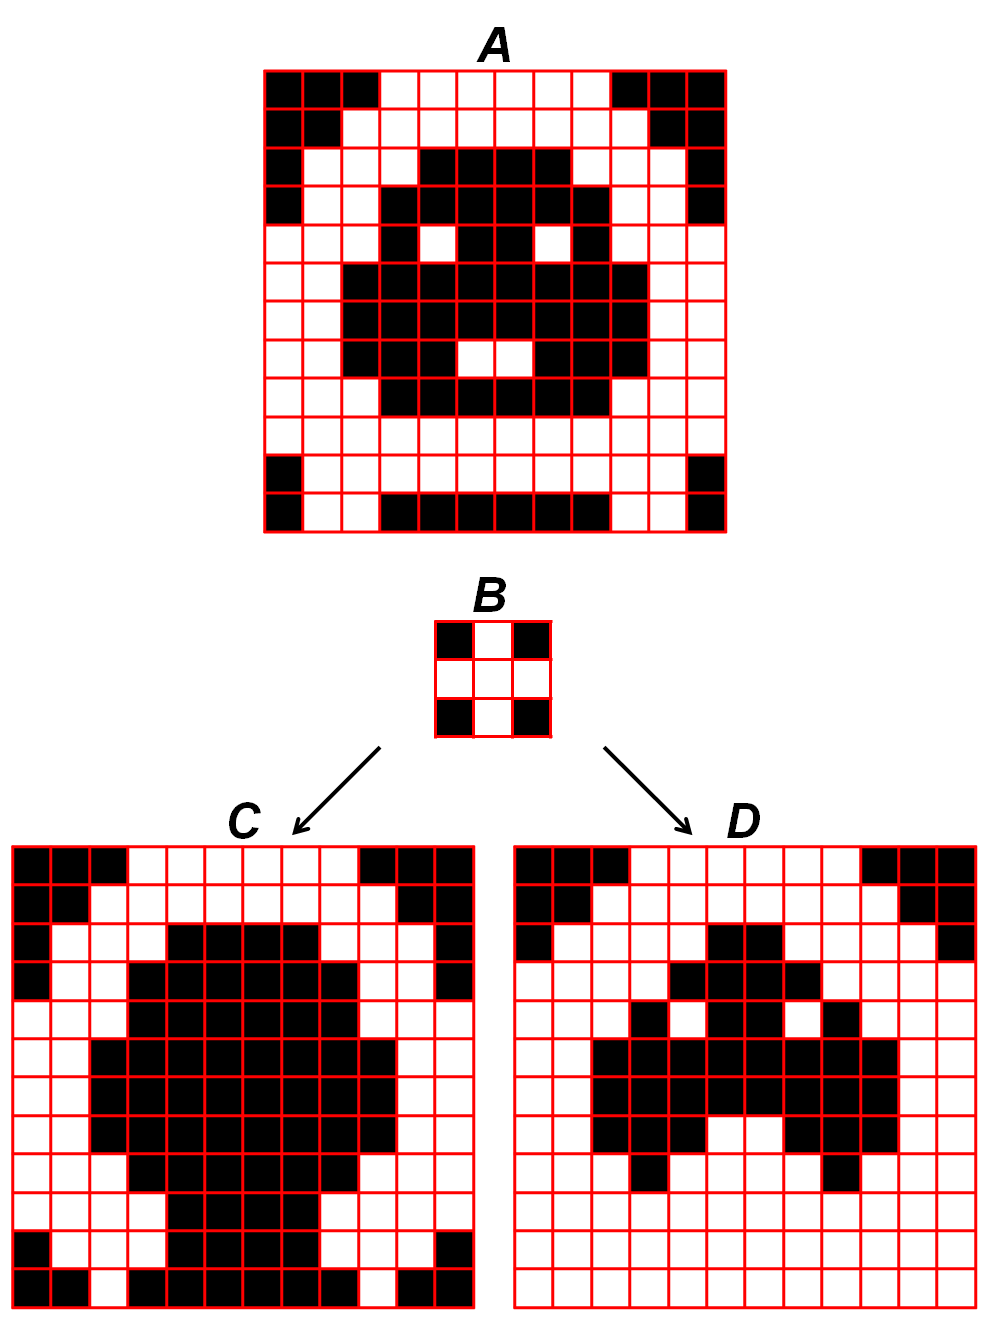
\includegraphics[height=334pt,width=250pt]{images/fig_open-close}
    \caption{Abertura e Fechamento.}\label{fig:open-close}
  \end{center}
\end{figure}

A \underline{abertura} de um conjunto \textit{\textbf{A}} por um
elemento estruturante \textit{\textbf{B}} (\textit{\textbf{A}} $\circ$
\textit{\textbf{B}}) é definida como:

\begin{align}
 &\textit{\textbf{A}} \circ \textit{\textbf{B}} = \left(\textit{\textbf{A}} \ominus \textit{\textbf{B}} \right) \oplus \textit{\textbf{B}} 
\end{align}

o que equivale a dizer que a abertura de \textit{\textbf{A}} por
\textit{\textbf{B}} é simplesmente a erosão de \textit{\textbf{A}} por
\textit{\textbf{B}} seguida de uma dilatação do resultado por
\textit{\textbf{B}}.

O \underline{fechamento} de um conjunto \textit{\textbf{A}} por um
elemento estruturante \textit{\textbf{B}} (\textit{\textbf{A}}
$\bullet$ \textit{\textbf{B}}) é definido como:

\begin{align}
  &\textit{\textbf{A}} \bullet \textit{\textbf{B}} =
  \left(\textit{\textbf{A}} \oplus \textit{\textbf{B}} \right) \ominus
  \textit{\textbf{B}}
\end{align}

ou seja, o fechamento não é mais que a dilatação de
\textit{\textbf{A}} por \textit{\textbf{B}} seguida da erosão do
resultado pelo mesmo elemento estruturante \textit{\textbf{B}}.

Como pode ser observado na Figura~\ref{fig:open-close}, a abertura em
geral suaviza o contorno de uma imagem, elimina faixas estreitas,
assim como objetos pequenos. Por sua vez, o fechamento pode preencher
trincas ou buracos pequenos e até conectar objetos próximos.

É bom ressaltar que estas operações morfológicas podem ser aplicadas
$k$ vezes sobre uma mesma imagem. Desta forma pode-se, por exemplo,
reduzir o tamanho de um objeto numa imagem binária através de
múltiplas erosões até chegar ao resultado desejado. Outro exemplo
poderia ser aplicar uma abertura de $k$ passos para eliminar pequenos
objetos espúrios.

A \underline{erosão derradeira} é um bom exemplo de iteração sucessiva
de operações morfológicas. Esta técnica consiste em simplesmente
erodir os objetos de uma imagem usando a Equação~\ref{eq-erode} até
que um próximo passo os eliminaria. Esta técnica pode ser utilizada,
por exemplo, para localizar ``sementes'' de objetos que mais tarde
viriam a ser usadas na segmentação por crescimento de
regiões.\cite{65}

O \underline{preenchimento de buracos} é outra das operação
morfológicas comumente utilizadas na análises de imagens. Neste caso,
entenda-se como buraco o interior de um subconjunto fechado
(contorno), de pixels brancos ($1$) de conectividade 8, que pertence
ao conjunto \textit{\textbf{A}}. Assim, partindo de um ponto $X_{0}$
situado dentro do contorno, o que se deseja é preencher o interior do
mesmo com pixels brancos. Assumindo que todos os pontos que não
pertencem ao contorno são pixels pretos ($0$), será atribuído o valor
$1$ a $X_{0}$ para iniciar o procedimento, e assim por todos os pontos
$X_{k}$ do interior contorno até preencher a região com pixels
brancos. Ou seja:

\begin{align}
 &X_{k} = \left(X_{k-1} \oplus \textit{\textbf{B}} \right) \cap \textit{\textbf{A}}^{c}
\end{align}

onde $k=1,2,3, ...$ e \textit{\textbf{B}} é o mesmo elemento
estruturante da Figura~\ref{fig:open-close}. O algoritmo termina na
$k$-ésima iteração se $X_{k}=X_{k-1}$.
 
O \underline{afinamento} é similar à erosão derradeira, porém com a
condição de não remover pixels que quebrariam o objeto em dois. Assim,
o afinamento de um conjunto \textit{\textbf{A}} por um elemento
estruturante \textit{\textbf{B}} (\textit{\textbf{A}} $\oslash$
\textit{\textbf{B}}) pode ser definido como:

\begin{align}
 &\textit{\textbf{A}} \oslash \textit{\textbf{B}} = \textit{\textbf{A}} \cap \left[ \left( \textit{\textbf{A}} \ominus b_{1}\right) \cap \left( \textit{\textbf{A}}^c \ominus b_{2}\right) \right]^{c}
\end{align}

onde \textit{\textbf{B}}=($b_1$,$b_2$) sendo que $b_1$ é o conjunto
dos elementos de \textit{\textbf{B}} associado com os pixels brancos e
$b_2$ é o conjunto dos elementos de \textit{\textbf{B}} associado com
os pixels pretos.

Até aqui, todas as operações morfológicas foram definidas usando um
elemento estruturante. Contudo, o uso de um elemento estruturante nem
sempre é a melhor escolha. O problema é que os elementos estruturantes
deformam os objetos, dando-lhes a forma deste elemento, transformando
contornos suaves em contornos angulosos. Porém, existem outras formas
de criar estes operadores morfológicos a partir do cálculo do Mapa de
Distâncias Euclidianas (MDE).

O \underline{MDE} é uma ferramenta, que diferentemente das operações
morfológicas anteriores, só pode ser usada em imagens binárias,
produzindo uma imagem em tom de cinza como imagem de saída.\cite{113}
A definição desta técnica é bastante simples, ela consiste em atribuir
um valor tonal a cada pixel proporcional à sua menor distância da
borda do objeto (Figura~\ref{fig:euclide-erode}b).

\begin{figure} [h]
  \begin{center}
    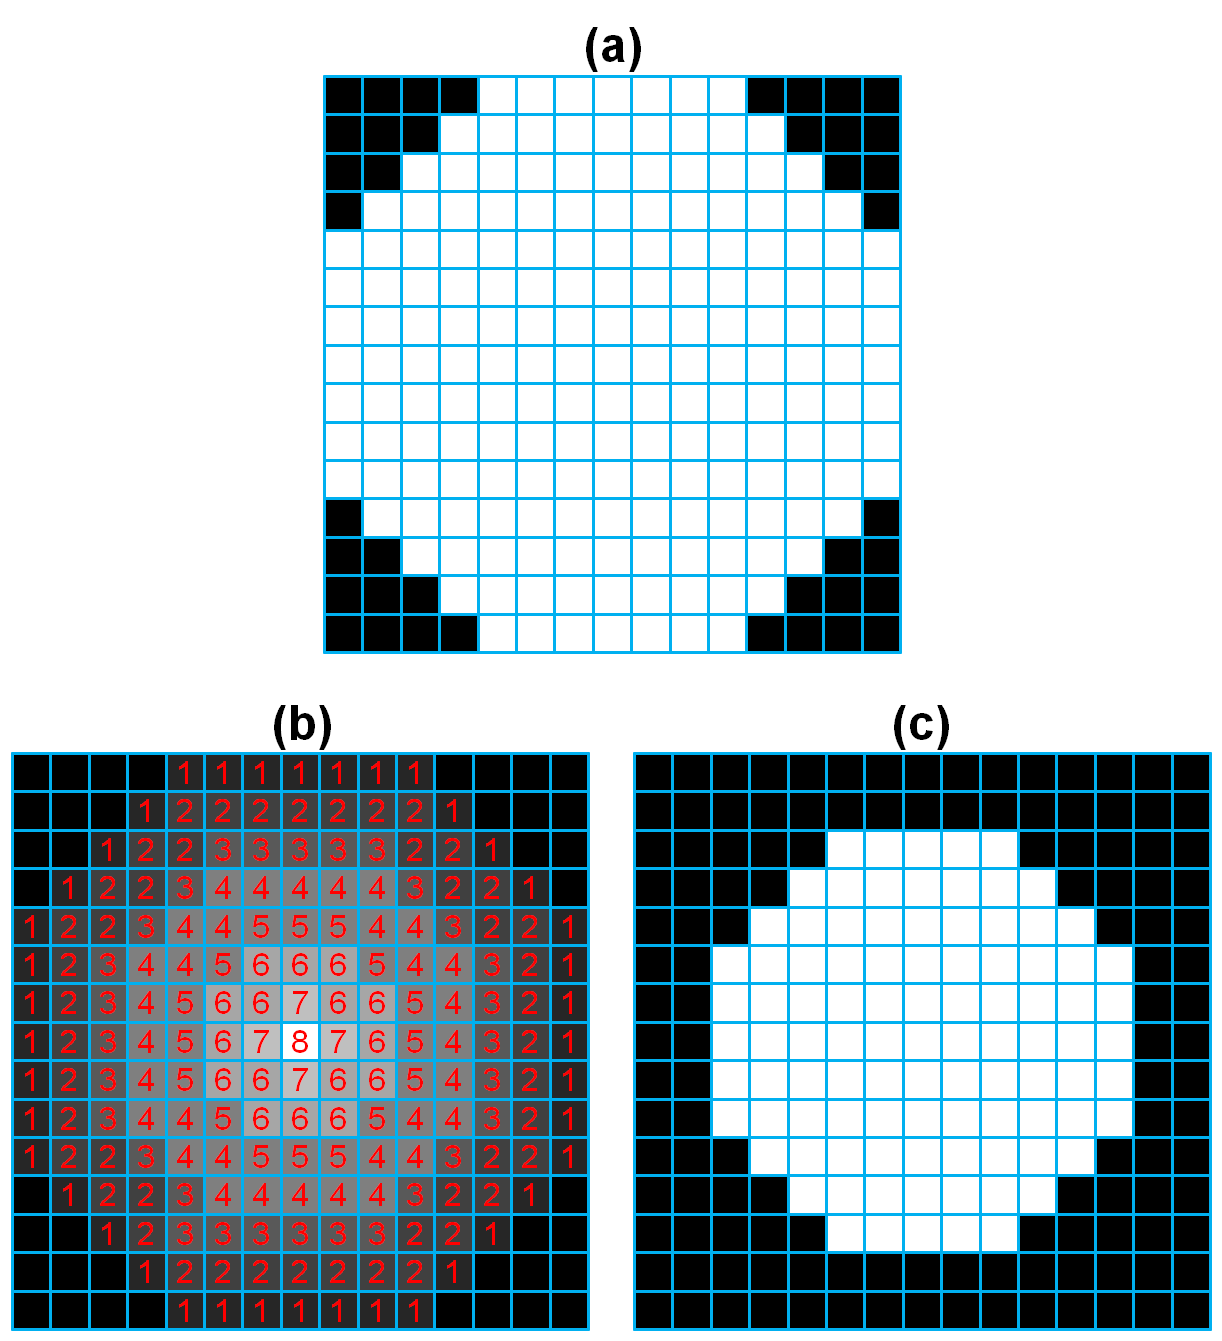
\includegraphics[height=274pt,width=250pt]{images/fig_euclide-erode}
    \caption{Exemplo esquemático do uso de MDE: (a) Imagem binária;
      (b) Imagem MDE; (c) Erosão de passo
      $2$.}\label{fig:euclide-erode}
  \end{center}
\end{figure}

Como pode ser observado na Figura~\ref{fig:euclide-erode}, a partir da
imagem binária de entrada (Figura~\ref{fig:euclide-erode}a), o calculo
do MDE gera uma imagem de saída em tons de cinza
(Figura~\ref{fig:euclide-erode}b), mantendo os pixels do fundo em
preto e atribuindo, a cada pixel dos objetos, o valor, aproximado ou
truncado, da distância euclideana deste pixel ao pixel mais próximo da
borda do objeto. A partir daqui, as operações morfológicas podem ser
feitas com uma simples linearização da imagem MDE. Foi assim que uma
erosão de passo $2$ foi aplicada nela, tomando como limiar inferior e
superior da segmentação os valores $1$ e $8$, respectivamente
(Figura~\ref{fig:euclide-erode}c).

No caso particular da dilatação, precisa-se inverter (NOT)
primeiramente a imagem binária, depois calcular o MDE, limiarizar o
MDE e finalmente inverter a imagem segmentada. Desta forma, com ajuda
da erosão e dilatação euclideanas, podem-se criar os operadores
morfológicos restantes.

As operações baseadas no MDE apresentam um custo computacional maior
que as anteriores. Contudo, este método realiza a propagação de
maneira verdadeiramente radial, afetando menos a forma dos objetos e
sendo independentes de sua rotação na imagem. De fato, as operações
morfológicas baseadas no MDE são mais acuradas.\cite{72}

Finalmente, outra operação morfológica que se baseia no MDE é o método
do divisor de águas.\cite{103} Este método é muito usado para separar
objetos que se tocam, ou parcialmente superpostos, na imagem. Este é
um problema muito comum, derivado de uma segmentação incompleta, o que
faz com que este método seja uma ferramenta muito importante na etapa
de pós-processamento.\cite{114}

O \underline{método do divisor de águas} se baseia no crescimento de
sementes dos objetos para visar sua separação. Para isto, calcula-se o
MDE (Figura~\ref{fig:euclide-watershed}b) da imagem binária de entrada
(Figura~\ref{fig:euclide-watershed}a). Este MDE será usado para obter
as sementes dos objetos (Figura~\ref{fig:euclide-watershed}c) através
de uma erosão derradeira da imagem binária de entrada. Finalmente, é
aplicada uma dilatação derradeira acima das sementes, porém com a
condição de que os objetos não voltem a se unir, para assim separar os
objetos (Figura~\ref{fig:euclide-watershed}d).

\begin{figure} [h]
  \begin{center}
    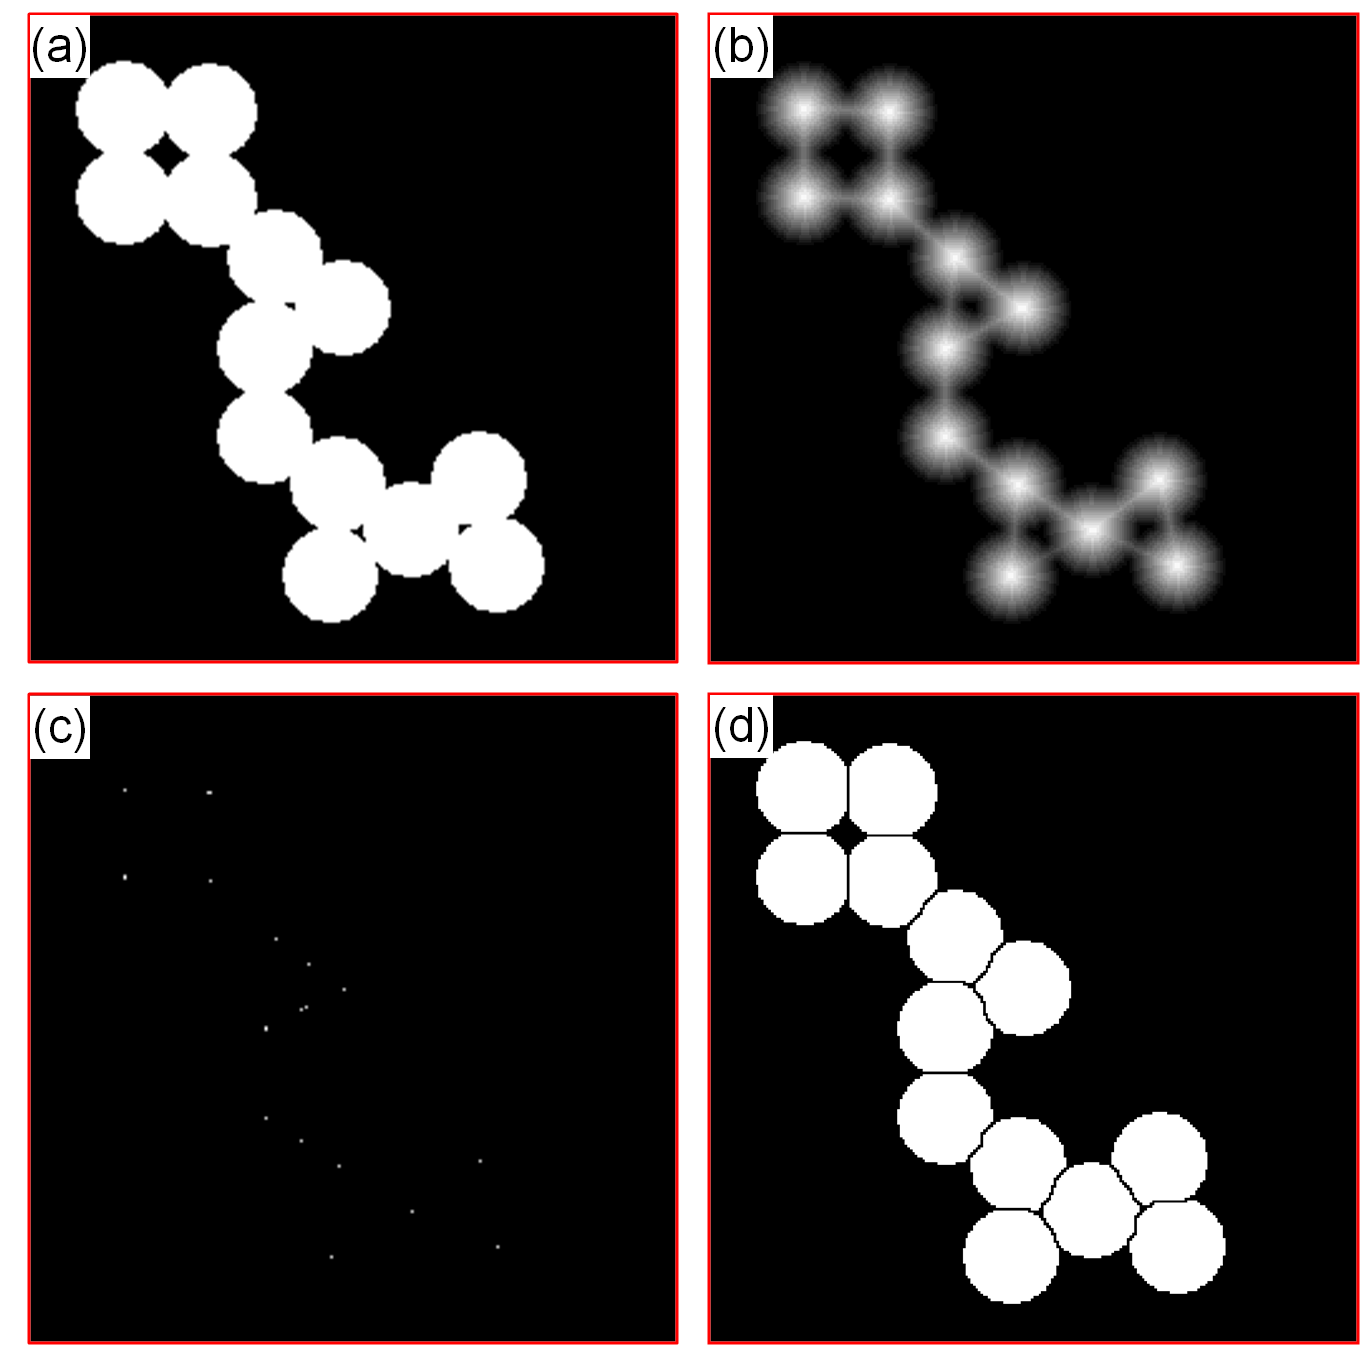
\includegraphics[height=346pt,width=350pt]{images/fig_euclide-watershed}
    \caption{Método dos divisores de água: (a) Imagem binária inicial;
      (b) Imagem MDE; (c) Imagem sementes; (d) Imagem binária com os
      objetos separados.}\label{fig:euclide-watershed}
  \end{center}
\end{figure}

Cada iteração da dilatação será equivalente à erosão anteriormente
sofrida, adicionando contornos com a espessura de um pixel à semente,
exceto aqueles pixels que eventualmente poderiam unir objetos. Este
processo permite que os objetos cresçam até seu tamanho original
conservando sua forma e separados por linhas de $1$ pixel de
espessura.

A ideia do nome ``método do divisor de águas'' surgiu pela aparente
topografia observada numa imagem MDE, que assemelha os objetos com
``montanhas'', onde quanto maior a distância de um pixel à borda do
objeto, maior será a sua ``altura''. Quando dois objetos se tocam,
formam-se dois picos, um vale entre eles é uma linha que os separa. A
ideia então seria fazer passar água pela linha com o fim de separar as
montanhas, daí o nome divisor de águas.

\subsection{Extração de Atributos}
%\label{sec:EA}

Na etapa de extração de atributos é onde fica mais marcada a diferença
entre processamento e análise de imagem. Nesta etapa é onde ocorre a
extração da informação dos objetos da imagem. Além disso,
características dos objetos e da imagem são medidas.\cite{114} Existem
basicamente duas classes de medidas:

\begin{enumerate}[label=(\roman{*})]
  \item Medidas de campo, que são as medidas feitas na imagem
    como um todo e
  \item Medidas de região, que são medidas feitas independentemente em
    cada objeto.
\end{enumerate}

Algumas das medidas de campo usadas com maior frequência são:

\begin{enumerate}[label=$\triangleright$]
  \item Contagem de objetos;
  \item Área total de objetos;
  \item Fração de área;
  \item entre outras.
\end{enumerate}

A contagem de objeto consiste em contar as regões de pixels contíguos
com a mesma tonalidade, que correspondem aos objetos numa imagem
binária. Este tipo de medida é o mais fácil de ser implementado, porém
problemas de conectividade podem eventualmente gerar erros
(Figura~\ref{fig:v4-v8}).

\begin{figure} [h]
  \begin{center}
    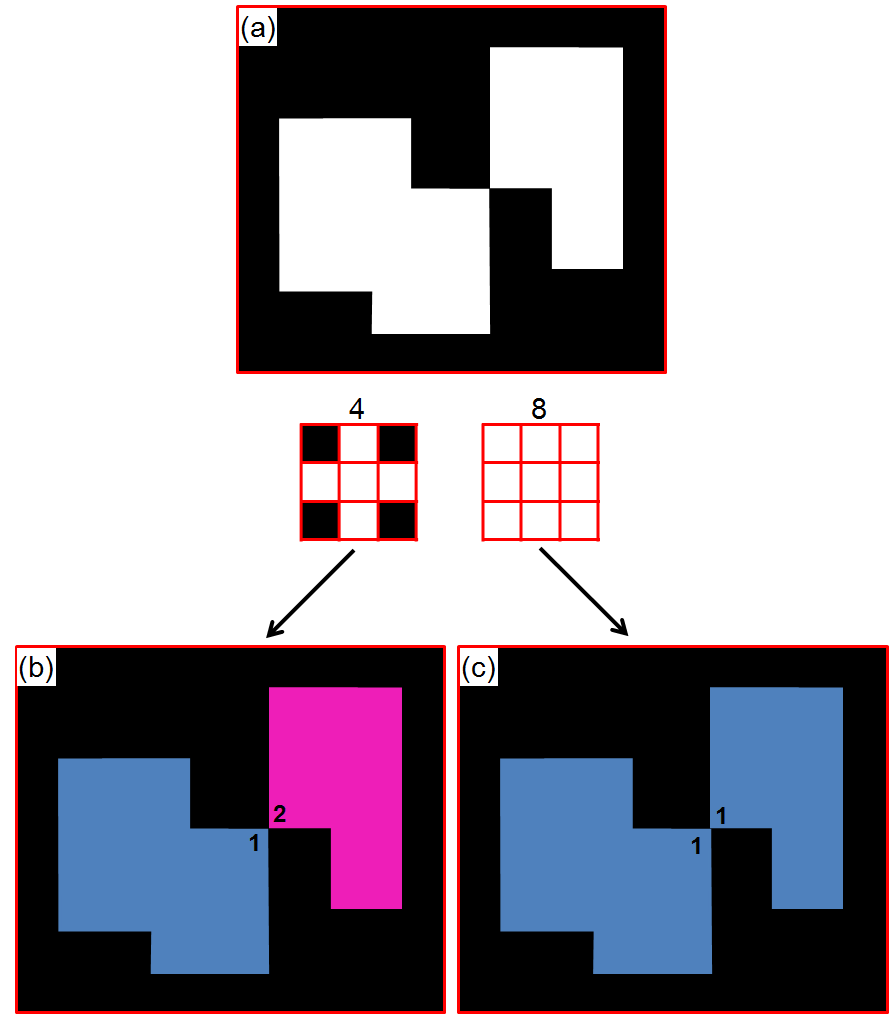
\includegraphics[height=342pt,width=300pt]{images/fig_v4-v8}
    \caption{Separação de objetos numa imagem binária dependendo do
      tipo de conectividade entre pixels: (a) Imagem binária inicial;
      (b) Objetos separados com conectividade 4; (c) Objetos não
      separados com conectividade 8.\cite{115}}\label{fig:v4-v8}
  \end{center}
\end{figure}

Este problema pode ser observado na Figura~\ref{fig:v4-v8}, onde uma
imagem binária tem dois objetos que se tocam
(Figura~\ref{fig:v4-v8}a). Estes objetos são separados em dois objetos
diferentes ($1$ e $2$) usando uma contagem de conectividade 4
(Figura~\ref{fig:v4-v8}b). Em contrapartida, o uso de uma
conectividade 8 leva a contagem de um objeto só
(Figura~\ref{fig:v4-v8}c). A escolha de qual conectividade usar vai
depender somente do problema em questão.
 
No caso da área total dos objetos, também é uma medida fácil de se
implementar, já que ela se baseia na contagem dos pixels brancos na
imagem binária. Esta área serve para calcular a fração de área do
campo ocupada por objetos. Para isto, calcula-se a razão entre o
número de pixels brancos (área total dos objetos) e o número total de
pixels (área da imagem) na imagem binária. Como pode ser notado, a
fração de área do campo é adimensional com valores entre $0$ e $1$.

Da mesma forma, nesta etapa são usadas medidas de região, tais como:
\begin{enumerate}[label=$\triangleright$]
  \item Área;
  \item Posição (Equação~\eqref{eq-centgrav});
  \item Perímetro (Equação~\eqref{eq-perim});
  %% \item Diâmetro Equivalente (Equação~\eqref{eq-diam}); 
  \item \textit{Ferets} (\textit{feret} máximo e mínimo);
  \item Razão de aspectos (Equação~\eqref{eq-ra});
  \item Fator de forma circular (Equação~\eqref{eq-ffc});
  \item Circularidade (Equação~\eqref{eq-ffcc});
  \item Convexidade (Equação~\eqref{eq-conv});
  \item Solidez (Equação~\eqref{eq-sol}); 
  \item entre outras.
\end{enumerate}

A Área ($A$), como nas medidas de campo, é calculada simplesmente
contando o número total de pixels de cada objeto da imagem
binária. Porém existem outras variantes de áreas, como área preenchida
e área convexa ($A_c$). A área preenchida é calculada da mesma forma
que a área, só que neste caso, também contam-se os pixels dos poros
internos aos objetos. Por sua vez a área convexa consiste na área
obtida após tornar o objeto convexo. Esta medida é equivalente à área
definida por um ``elástico'' passado em torno do objeto.

A posição de um objeto numa imagem binária pode ser descrita por
várias formas diferentes, umas mais simples de serem calculadas que as
outras. Por exemplo, as coordenadas de seu centro de gravidade e as
medidas relativas ao retângulo circunscrito, ou seja, as maiores e
menores coordenadas dos pixels nas direções horizontais e
verticais. Não entanto, as medidas relativas ao retângulo circunscrito
podem ser muito sensíveis a possíveis rotações dos objetos, assim as
coordenadas do centro de gravidade ($CG_x,CG_y$) descrevem melhor a
posição do objeto.\cite{114} Ou seja:

\begin{align}\label{eq-centgrav}
 \begin{array}{c c c}
  &CG_x=\dfrac{\sum\limits_{i=1}^n{x_i}}{Area}\\
  ~\\[-3mm]
  &CG_y=\dfrac{\sum\limits_{i=1}^n{y_i}}{Area}
 \end{array}
\end{align}

onde $x_i$ e $y_i$ são as coordenadas do \textit{i-ésimo} pixel e
$Area$ é o número total de pixels brancos do objeto.

Por outro lado, o perímetro pode ser calculado somando o número de
``passos'' na horizontal, vertical ou diagonal dados de cada pixel
para o seguinte até percorrer todo o contorno do objeto da imagem
binária. Ou seja:

\begin{align}
 &P=N+\sqrt{2}N_{d}\label{eq-perim}
\end{align}

onde $N$ é o número de passos horizontais ou verticais e $N_{d}$ é o
número de passos diagonais. No caso do perímetro, o perímetro dos
poros internos do objeto também são considerados. Em contrapartida, no
caso do perímetro preenchido só é considerado o perímetro do contorno
do objeto. Finalmente no perímetro convexo ($P_c$) só é considerado o
perímetro do ``elástico'' passado em torno do objeto.

Um exemplo do cálculo do perímetro pode ser observado na
Figura~\ref{fig:eq-perim}. Neste caso $N=12+4=16$ passos e
$N_{d}=16+4=20$ passos, então $P=16+20\sqrt{2}=44,3$ passos. Desta
forma pode-se dizer que, segundo a Equação~\eqref{eq-perim}, o
perímetro do objeto é de $44,3$ pixel.

\begin{figure} [h]
  \begin{center}
    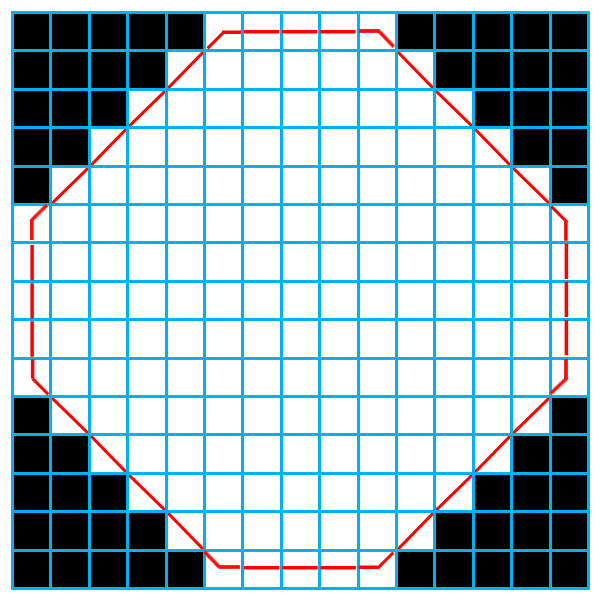
\includegraphics[height=150pt,width=150pt]{images/fig_eq-perim}
    \caption{Cálculo do perímetro de um objeto através dos passos
      horizontais, verticais e diagonais.}\label{fig:eq-perim}
  \end{center}
\end{figure}

% Da mesma forma, pode-se definir o diâmetro equivalente de um
% objeto. Este diâmetro é definido como o diâmetro equivalente de um
% circulo com igual área do objeto de interesse. Ou seja:

%\begin{align} 
% &Diam=2\sqrt{\frac{Area}{\pi}}\label{eq-diam}
%\end{align}

Os \textit{ferets} máximos e mínimos equivalem às projeções máximas e
mínimas do objeto, caracterizando assim sua dimensão externa. Por sua
vez, a razão entre o \textit{feret} mínimo e \textit{feret} máximo é
uma boa medida do alongamento do objeto. Ou seja:

\begin{align} 
 &RA=\dfrac{F_{min}}{F_{max}}\label{eq-ra}
\end{align}

onde $F_{min}$ é o \textit{feret} mínimo e $F_{max}$ é o
\textit{feret} máximo.

Por sua vez, o fator de forma circular parte da relação que existe
entre o perímetro e a área de um círculo ($P^2 = 4 \pi A$). Esta
relação só será uma igualdade para o caso do círculo, já para qualquer
outra forma geométrica do objeto teremos que $P^2 > 4 \pi A$. Desta
relação surge o fator de forma circular como:

\begin{align}
 &FFC=\dfrac{4\pi A}{P^{2}}\label{eq-ffc}
\end{align} 

que é uma boa medida da suavidade dos contornos dos objetos, devido a
sua forte dependência do perímetro. Onde $A$ é a área preenchida e $P$
é o perímetro obtido pela Equação~\eqref{eq-perim}. Caso se deseje um
fator de forma circular mais sensível ao alongamento do objeto e menos
dependente da suavidade do contorno, então basta substituir $P^2$ por
$(\pi F_{max})^2$, como:

\begin{align}
 &FFC_c=\dfrac{4 A}{\pi (F_{max})^{2}}\label{eq-ffcc}
\end{align}

onde $A$ é a área preenchida e $F_{max}$ é o \textit{feret}
máximo. Este novo fator de forma circular é chamado de circularidade
($FFC_c$). Outras variantes do fator de forma circular são:

\begin{align}
 &FFC_m=\dfrac{4 A}{P (F_{max})}\label{eq-ffcm}
\end{align}

e

\begin{align}
 &FFC_g=\dfrac{16 A^{2}}{\pi P(F_{max})^{3}}\label{eq-ffcg}
\end{align}

onde $FFC_m$ é chamado de fator de forma circular
modificado.\cite{121} Da mesma forma, $FFC_g$ é chamado de fator de
forma circular grum.\cite{502}

Finalmente os objetos podem ser definidos por sua concavidade através
da convexidade ($C$) e da solidez ($S$), de modo que:

\begin{align}
 &C=\dfrac{P_{c}}{P}\label{eq-conv}
\end{align} 

e

\begin{align}
 &S=\dfrac{A}{A_{c}}\label{eq-sol}
\end{align} 

onde, $P_{c}$ e $A_{c}$ são o perímetro e a área convexa, respectivamente.

Como já deve ter sido notado, os fatores de forma são adimensionais
derivados das medidas geométricas básicas (área, perímetro,
\textit{ferets}, etc). Eles geralmente tem valores entre $0$ e $1$,
sendo $1$ para formas padrões (geométricas regulares) e valores
menores para formas irregulares. No caso do $FFC$ vale $1$ para
objetos circulares e apresenta valor menor para objetos com outras
formas.

A fim de caracterizar a forma de um objeto a partir do conceito de
alongamento são utilizados alguns fatores adimensionais de forma mais
genéricos, que não visam comparar sua forma a um modelo específico. Um
destes fatores de forma é a $RA$, a mesma é inversamente proporcional
ao alongamento, sendo igual a $0$ quando ele tende ao infinito.

Também é possível descrever um objeto como côncavo ou convexo com os
fatores de forma $C$ e $S$, o primeiro dependente do perímetro e o
segundo da área. Estes fatores de forma têm valores iguais a $1$
quando o objeto é convexo e diminuem com a presença da concavidade. Ao
mesmo tempo, por depender do perímetro, $C$ é mais sensível à
suavidade do contorno que $S$.

Na Figura~\ref{fig:compara-factform} pode-se observar a influência das
propriedades de alongamento e suavidade do contorno em alguns fatores
adimensionais de forma.\cite{114} Nota-se que os objetos da esquerda
(A, C e E) são facetados, enquanto que os à direita (B, D e F) possuem
contornos mais suaves. Assim, os objetos A, C e E apresentaram valores
próximos a $0,32$ e $0,72$ no fator de forma circular e convexidade,
respectivamente. Os objetos B, D e F apresentaram valores próximos a
$0,47$ e $0,81$, para esses mesmos parâmetros. Além disso, o
alongamento dos objetos diminui de cima para baixo, de modo que há
claramente três níveis de razão de aspecto, característicos para os
pares A-B, C-D, e E-F.\cite{72,114}

\begin{figure} [h]
  \begin{center}
    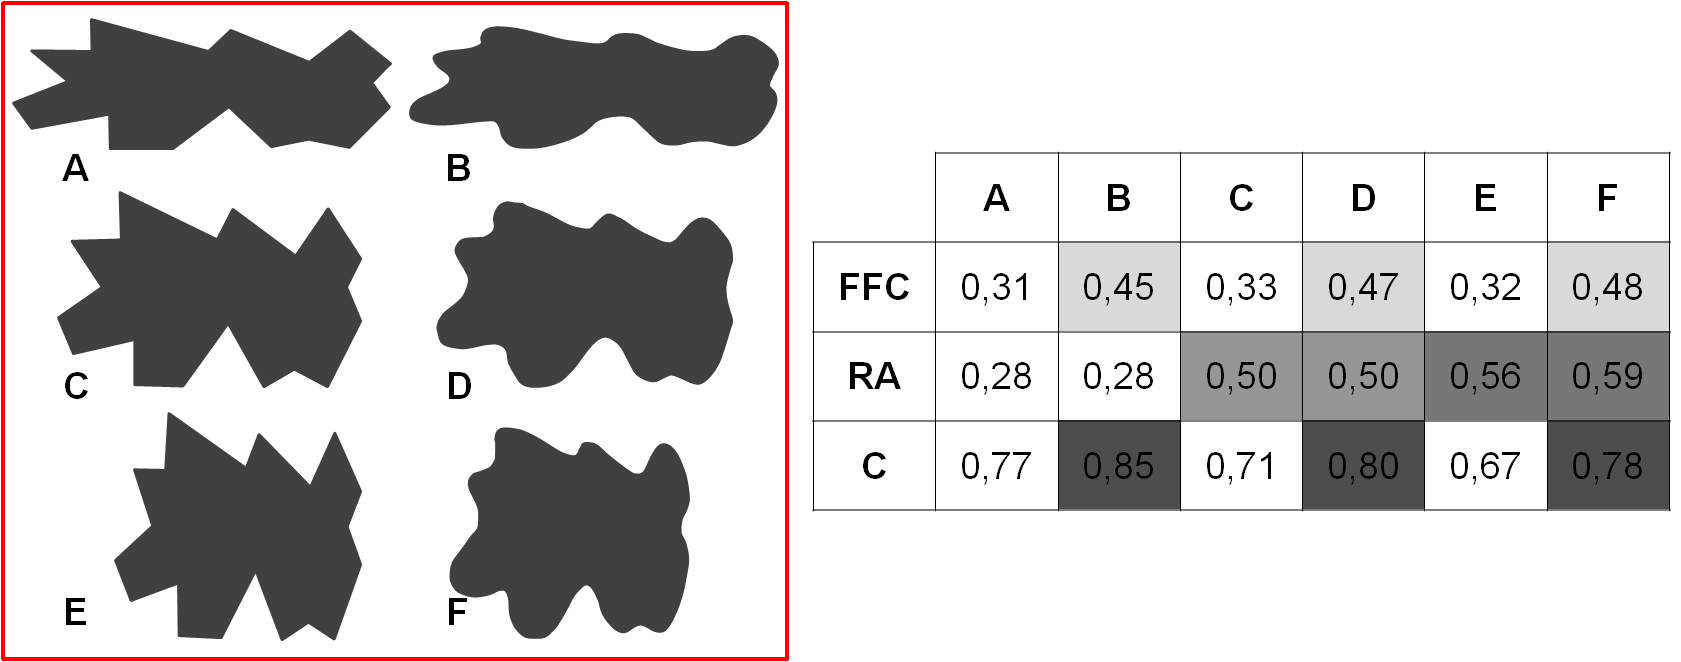
\includegraphics[height=157pt,width=400pt]{images/fig_compara-factform}
    \caption{Comparação de fatores adimensionais de
      forma.\cite{114}}\label{fig:compara-factform}
  \end{center}
\end{figure}

\vspace{20 mm}

\subsection{Reconhecimento e Classificação}

A etapa de reconhecimento e classificação é a etapa final da sequência
padrão de PADI. Durante essa etapa é realizado o tratamento dos dados
quantitativos obtidos na etapa anterior, interpretando-os, de modo a
fornecer um resultado de mais alto nível, similar ao processo de
reconhecimento de padrões realizado pelo cérebro humano.

Segundo o dicionário Houaiss, a definição da palavra ``reconhecer'' é
tomar conhecimento de novo ou em outra situação, distinguir os traços
característicos de alguém ou algo; caracterizar, identificar,
distinguir (alguém ou algo) por certos caracteres.\cite{116} O
reconhecimento pode-se acontecer por identidade ou por semelhança. No
reconhecimento por identidade um objeto, previamente conhecido, é
identificado. Por outro lado, o reconhecimento por semelhança ocorre
quando um objeto é identificado como membro de uma classe através de
traços característicos. Deste modo, o reconhecimento pode ser visto
como um processo de classificação.\cite{30}

As técnicas de reconhecimento de padrões são usadas para classificar
objetos através de um conjunto de propriedades ou características
comuns a cada classe de objetos.\cite{117} O reconhecimento de padrões
por computadores é parte importante da inteligência artificial. Estes
sistemas bem podem ser usados por uma pessoa para restringir sua
atenção a um conjunto de casos selecionados pelo sistema, ou bem para
automatizar completamente o processo de tomada de decisão, sem
necessidade de intervir pessoalmente.\cite{30}

O crescimento acelerado e disponibilidade de capacidade computacional
tornam mais rápido o processamento de grandes conjuntos de dados, além
de facilitar o uso de métodos elaborados e variados para análise e
classificação destes dados. Computadores, às vezes, são melhores
classificadores que as pessoas, devido a que eles não se distraem com
variações aleatórias de parâmetros não críticos e conseguem extrair
comportamentos estatísticos significativos para isolar
grupos.\cite{114}

Em contrapartida, as pessoas geralmente ainda são mais rápidas no
reconhecimento de padrões que os computadores.\cite{114} Ao mesmo
tempo, a quantidade de dados a serem processados vem aumentando com o
tempo, o que tem gerado também um aumento da demanda por melhorias no
desempenho das técnicas de reconhecimento de padrões, tanto em
velocidade como em exatidão e custo.

Um padrão pode ser descrito matematicamente como um vetor cujas
componentes são características numéricas dos objetos de interesse, as
quais são obtidas por meio de um conjunto de
observações.\cite{118,119} O problema de reconhecimento é colocado
como uma tarefa de classificação ou categorização dos padrões.

Por outro lado, as classes são definidas como um conjunto de padrões
semelhantes entre si. Estas classes podem ser identificadas como
regiões do espaço de características onde é muito provável encontrar
pontos representativos dos objetos. Isto significa que quando são
extraídas as características de um conjunto de objetos pertencentes à
mesma classe, os pontos representativos destes no espaço de
características devem agrupar-se mantendo entre si distâncias menores
do que aquelas que se medem em relação a objetos pertencentes a outras
classes. Desta forma são formados agrupamentos, aglomerados ou
\textit{clusters}.\cite{30}

Os sistemas de classificação são divididos, conforme a participação ou
não do usuário, em supervisionados ou não supervisionados
(Figura~\ref{fig:class-supnaosup}).\cite{119} Os sistemas de
classificação supervisionados são aqueles em que o usuário define as
classes rotulando objetos que lhe são apresentados. Neste caso, as
classes são conhecidas ou previamente determinadas pelo usuário do
sistema de classificação. Os sistemas de classificação
não-supervisionados são aqueles em que a semelhança entre os padrões é
estabelecida pelo sistema, o qual identifica quantas e quais são as
classes. Este tipo de sistema é usado quando as classes são
desconhecidas ou precisa-se de um sistema de classificação sem a
intervenção do usuário.\cite{52}

\begin{figure} [h]
  \begin{center}
    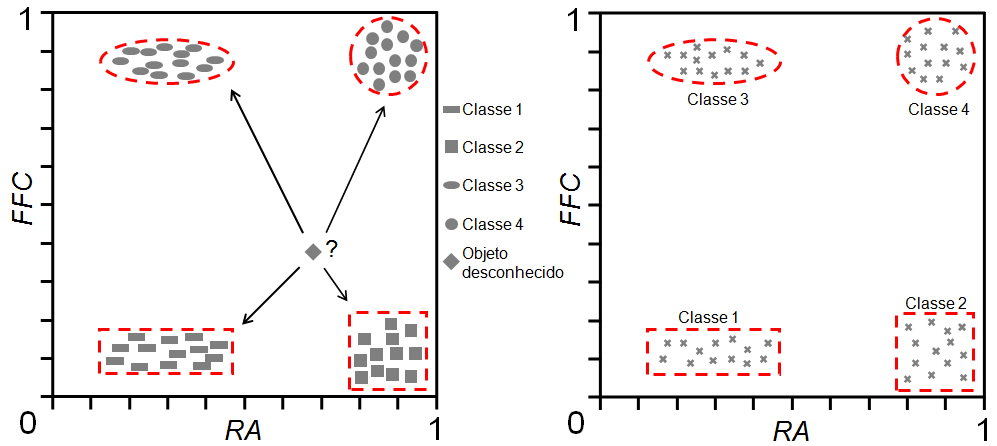
\includegraphics[height=179pt,width=400pt]{images/fig_class-supnaosup}
    \caption{Tipos de sistemas de classificação utilizando os
      parâmetros característicos FFC e RA: (a) Classificação
      supervisionada; (b) Classificação
      não-supervisionada.}\label{fig:class-supnaosup}
  \end{center}
\end{figure}
 
A Figura~\ref{fig:class-supnaosup}a ilustra um sistema
supervisionado. Nela pode-se observar um conjunto de objetos
representados em um espaço de características bidimensional (razão de
aspecto vs. fator de forma circular). Como a legenda indica, estes
objetos são conhecidos e foram previamente rotulados (classe 1, classe
2, classe 3 e classe 4). Tanto a morfologia dos objetos quanto o
espaço de características bidimensional foram escolhidos
intencionalmente assim. Desta maneira o objeto desconhecido fica mais
próximo da classe 2 que do resto, como indicam os comprimentos das
setas (distância à classe 2 $<$ distância à classe 1 $<$ distância à
classe 4 $<$ distância à classe 3).
 
Assim, a partir desta base de conhecimento, pode ser atribuída uma
classe a um objeto desconhecido através de um procedimento de
classificação supervisionada. Portanto, o objeto desconhecido é
classificado como pertencente à classe 2. O critério utilizado é a
proximidade, no espaço de características, aos objetos desta classe.

A Figura~\ref{fig:class-supnaosup}b mostra a classificação
não-supervisionada. Neste caso, os padrões dos objetos são
desconhecidos. Contudo, um procedimento de classificação
não-supervisionada procura por objetos similares e os agrupa em
classes. Neste caso, apesar de não conhecer a morfologia dos objetos,
o classificador consegue separá-los em quatro classes diferentes, como
no exemplo anterior. Contudo, os sistemas não-supervisionados escapam
do escopo deste trabalho.

\subsubsection{Conjunto de treinamento}

O conjunto de treinamento é um conjunto de objetos previamente
identificado pelo usuário. Este conjunto de treinamento deve ser
estatisticamente grande, com o intuito de aumentar a precisão do
classificador, além de apresentar grande variabilidade dentro de cada
classe para assim poder garantir uma boa representatividade.

Como poderá ser observado mais na frente, o conjunto de treinamento
precisa crescer exponencialmente com o aumento da dimensionalidade do
espaço de características.\cite{120} Outros autores definem que o
conjunto de treinamento deve aumentar em dez vezes por classe, com o
aumento da dimensionalidade do espaço de características.\cite{119}
Contudo, nem sempre é possível obter mais objetos conhecidos para
ampliar o conjunto de treinamento.

\subsubsection{Conjunto de características}

A escolha do conjunto de características é feita a partir da
observação dos atributos que melhor representam as classes no conjunto
de treinamento. O conjunto de atributos que define o espaço de
características deve caracterizar bem os objetos, agrupando os objetos
similares e separando os distintos. Este conjunto deve ser sensível o
bastante para descriminar todas as classes.

Raramente uma única característica separa mais de duas classes, sendo
geralmente utilizadas várias características. Porém, um número de
características muito grande em relação ao tamanho do conjunto de
treinamento pode acarrear problemas de dimensionalidade. Um espaço de
características com dimensionalidade muito alta torna o sistema mais
complexo, consumindo maior tempo no treinamento e ainda podendo
reduzir a capacidade de generalização do sistema.\cite{121} Assim, é
de crucial importância realizar uma cuidadosa escolha do conjunto de
características.

Na verdade, a alta dimensionalidade é um problema bastante recorrente
no reconhecimento de padrões, chegando a ser chamada de ``maldição da
dimensionalidade''. Assim, várias técnicas foram desenvolvidas com o
intuito de reduzir a dimensionalidade do espaço de características com
a esperança de obter problemas mais simples. Um exemplo disto é a
Análise Discriminante Linear (LDA).\cite{120}

Fica claro que a dimensionalidade poderia ser reduzida de $d$
dimensões para $1$ dimensão se for possível projetar as $d$ dimensões
numa linha formando \textit{clusters} devidamente separados. Este é
exatamente o objetivo da análise discriminante linear, que serve de
base para as técnicas de Análise Discriminante de Fisher (FDA) e a
Análise de Componentes Principais (PCA), também conhecida como
Transformada de Karhunen-Loève (KLT). Estes métodos são dos mais
populares usados para a redução da dimensionalidade, porém outros
métodos como o Escalonamento Multidimensional (MDS) também podem ser
úteis.\cite{117,122} No presente trabalho foram usadas as técnicas PCA
e FDA.

\vspace{20 mm}

\subsubsection{Classificadores}

Os classificadores são funções que utilizam como entrada os padrões
desconhecidos, e como saída as classes a que estes padrões
provavelmente pertencem. Os classificadores podem ser divididos em
dois tipos principais: os estatísticos (paramétricos e não
paramétricos) e os conexionistas (redes neurais).\cite{52}

Os classificadores estatísticos não paramétricos são os mais
simples. Eles utilizam uma função de distância como medida de
similaridade, atribuindo um objeto desconhecido à classe mais próxima
dele no espaço de características. Dois dos classificadores não
paramétricos comumente empregados são o de Distância Euclideana e o de
Distância de Mahalanobis.

Antes de entrar em detalhes acerca dos classificadores estatísticos,
serão definidas algumas nomenclaturas e conceitos a serem usados. Seja
$w_1,w_2,...,w_W$ um padrão de classe que contem algumas propriedades
em comum, onde $W$ é o número total de classes. Da mesma forma
\textbf{x} é um padrão de características, que não é mais que um vetor
de $n$ componentes:

\begin{align}\label{eq-meadclass}
 &\textbf{x}=
  \left[ 
   \begin{array}{c c c c c c}
    x_1\\[-2mm]
    x_2\\[-4mm]
    .\\[-5mm]
    .\\[-5mm]
    .\\[-1mm]
    x_n
   \end{array}  
  \right]
\end{align}

onde cada componente, $x_k$, representa a $k$-ésima medida de um total
de $n$ medidas (Seção~\ref{sec:Extração de Atributos}) associadas ao padrão.

Para finalizar, será definida a função discriminante ($d$) que vai
separar as classes ($w$) decidindo a que classe pertence um
determinado padrão de características. Assim, a fronteira de separação
entre as classes $w_i$ e $w_j$ será dada pelo valor \textbf{x} para o
qual:

\begin{align}
 &d_{i}(\textbf{x})=d_{j}(\textbf{x})
\end{align}

ou seja,

\begin{align}
 &d_{i}(\textbf{x})-d_{j}(\textbf{x})=0
\end{align}

Assim, é uma prática comum identificar a fronteira de separação entre
duas classes como:

\begin{align}\label{eq-dij}
 &d_{ij}(\textbf{x})=d_{i}(\textbf{x})-d_{j}(\textbf{x})=0
\end{align}

Desta forma $d_{ij}(\textbf{x})>0$ para objetos pertencentes à classe
$w_i$ e $d_{ij}(\textbf{x})<0$ para objetos pertencentes à classe
$w_j$. Tendo claro estes conceitos, pode-se detalhar alguns
classificadores de interesse.

O classificador de Distância Euclideana, também conhecido como
classificador de distância mínima, consiste em primeiramente calcular
a média da classe $w_i$:

\begin{align}\label{eq-meadclass}
 &\bar{\textbf{x}}_i=\dfrac{1}{N_i}\sum\limits_{i=1}^W{\textbf{x}_i}
\end{align}

onde $N_i$ é o número total de padrões de características pertencentes
à classe $w_i$. Assim, para determinar a classe a qual pertence um
padrão de características desconhecido \textbf{x}, calcula-se a
distância mínima ou distância euclideana da seguinte forma:

\begin{align}
 &D_i(\textbf{x})=\parallel \textbf{x}-\bar{\textbf{x}}_i \parallel
\end{align}

então:

\begin{align}\label{eq-euclidist}
 &D_i^2(\textbf{x})=\left(\textbf{x} - \bar{\textbf{x}}_i\right)^{T} \left(\textbf{x} - \bar{\textbf{x}}_i\right)
\end{align}

Deste modo, o objeto será atribuído à classe mais próxima
dele. Fazendo uso da definição de função discriminante e da
Equação~\ref{eq-euclidist}, após algumas simplificações temos que:

\begin{align}\label{eq-di}
 &d_i(\textbf{x})= \textbf{x}^{T}\bar{\textbf{x}}_{i}-\dfrac{1}{2}\bar{\textbf{x}}_{i}^{T}\bar{\textbf{x}}_{i}
\end{align}

Finalmente, das Equações~\ref{eq-dij} e~\ref{eq-di}, a função
discriminante que vai separar as classes $w_i$ e $w_j$ através do
classificador de distâncias euclideana é:

\begin{align}\label{eq-fundiscri}
 &d_{ij}(\textbf{x})= \textbf{x}^{T}\left(\bar{\textbf{x}}_{i} - \bar{\textbf{x}}_{j}\right)-\dfrac{1}{2}\left(\bar{\textbf{x}}_{i} - \bar{\textbf{x}}_{j}\right)^{T}\left(\bar{\textbf{x}}_{i} - \bar{\textbf{x}}_{j}\right)=0
\end{align}

Como pode ser observado, o classificador de distância euclideana só dá
garantias de bons resultados caso todas as classes tenham a mesma
variância em todas as características. É assim que o classificador de
distância de Mahalanobis, embora seja muito parecido ao de distância
euclideana, atende melhor este problema. Para isto, ele normaliza a
distância subtraindo cada característica por sua média e dividindo-a
pelo desvio padrão, segundo:

\begin{align}
&\bar{x} = \dfrac{\left| x-\mu \right|}{\sigma}
\end{align}

Desta modo, generalizando para um padrão de características, obtém-se
a distância de Mahalanobis de forma similar à
Equação~\ref{eq-euclidist}, ou seja:

\begin{align}
 &D_i^2(\textbf{x})=\left(\textbf{x} - \bar{\textbf{x}}_i\right)^{T} \Sigma_{i}^{-1} \left(\textbf{x} - \bar{\textbf{x}}_i\right)
\end{align}

onde $\Sigma_{i}$ é a matriz de covariância da classe $w_{i}$,
definida como:

\begin{align}\label{eq-covariancia}
 &\Sigma_{i}=\dfrac{1}{(N_{i}-1)}\sum\limits_{i=1}^W{\left(\textbf{x} - \bar{\textbf{x}}_{i}\right)\left(\textbf{x} - \bar{\textbf{x}}_{i}\right)^{T}}
\end{align}

onde $N_i$ é o número total de padrões de características pertencentes
à classe $w_i$.

Um dos classificadores estatísticos paramétricos mais usados é o
classificador de Bayes, também conhecido como classificador
bayesiano. Este consiste em minimizar a probabilidade média de erro
total na classificação.\cite{88} Assim, seja $P(w_i)$ a probabilidade
a \textit{priori} de ocorrência da classe $w_i$ ($i=1,2,...,W$), tal
que:

\begin{align}
 &\sum\limits_{i=1}^{W}P(w_i)=1
\end{align}

e $p(\textbf{x}|w_i)$ a densidade de probabilidade de uma
características $\textbf{x}$ que vem de uma classe $w_i$ conhecida,
então $p(\textbf{x})$ seria a densidade de probabilidade de uma
características $\textbf{x}$ que vem de uma classe desconhecida. Assim
temos que:

\begin{align}\label{eq-densprobx}
 &p(\textbf{\textbf{x}})=\sum\limits_{i=1}^{W}p(\textbf{\textbf{x}}|w_i)P(w_i)
\end{align}

Por sua vez, conhece-se da teoria clássica das probabilidades que:

\begin{align}\label{eq-probwx}
 &P(w_{i}|\textbf{x})=\dfrac{p(\textbf{x}|w_i)P(w_{i})}{p(\textbf{x})}
\end{align}

Assim, as regras de classificação de Bayes podem começar a ser
definidas como:

\begin{align}\label{eq-bayesreglas1}
 \begin{array}{c c}
  &\text{Se } P(w_{1}|\textbf{x})>P(w_{2}|\textbf{x}), \:\:\: \text{\textbf{x} pertence à classe $w_1$}\\
  &\text{Se } P(w_{1}|\textbf{x})<P(w_{2}|\textbf{x}),\:\:\: \text{\textbf{x} pertence à classe $w_2$}
 \end{array}
\end{align}

Usando a Equação~\ref{eq-probwx}, as regras ficam como:

\begin{align}\label{eq-bayesreglas2}
  \begin{array}{c c}
    &\text{Se } p(\textbf{x}|w_{1})P(w_1)>p(\textbf{x}|w_{2})P(w_2), \:\:\: \text{\textbf{x} pertence à classe $w_1$}\\
    &\text{Se } p(\textbf{x}|w_{1})P(w_1)<p(\textbf{x}|w_{2})P(w_2),\:\:\: \text{\textbf{x} pertence à classe $w_2$}
 \end{array}
\end{align}

onde $p(x)$ não foi levado em consideração já que é o mesmo para todas
as classes e isto não afeta à decisão. Assim, finalmente, podemos
definir a função discriminante de Bayes como:

\begin{align}\label{eq-dibayes}
 &d_i(\textbf{x})= p(\textbf{x}|w_{i})P(w_i)
\end{align}

Estes são alguns exemplos de classificadores estatísticos comumente
utilizados. No final, a escolha de tipo de classificador vai depender
do problema em questão e do que estiver disponível no software.

Por outro lado, os classificadores conexionistas são redes neurais
artificiais. As redes neurais constituem classificadores mais
complexos, inspirados na estrutura neural de organismos inteligentes,
que aprendem por experiência.\cite{52} Classificadores baseados nas
redes neurais possuem capacidade de se ajustar a qualquer topologia de
classes, o que os tornam muito eficientes nos casos onde há classes
com distribuições mal-comportadas.\cite{88} Contudo, para os problemas
de classificação deste trabalho, os classificadores estatísticos são
eficazes. Deste modo, as redes neurais não fazem parte do escopo deste
trabalho.
